%to do: slide 15, reduce number of variables
% slide 10, seperate a_t and b_t figures, give a_t first



%\documentclass[12pt,reqno,utf8,utf8x]{article}

\documentclass[8pt,aspectratio=169]{beamer}
\usepackage{natbib}
\usepackage{tikz}

%\usetheme[progressbar=frametitle]{metropolis}
\usepackage[utf8]{inputenc}
\usepackage{graphicx}
\usepackage{animate}
\graphicspath{ {images/} }
\usepackage{geometry}
\usepackage{subfigure}
\usepackage[english]{babel}
\usepackage[]{xcolor}
\usepackage{sansmathaccent}
\usepackage{amsmath,amsfonts,amssymb}
\usepackage{verbatim}
\usepackage{gensymb}
\usepackage{bm}
\usepackage{float}
\usepackage{rotating}
\usepackage{graphicx}
\usepackage{setspace}
\numberwithin{equation}{section}
\usepackage{fancyhdr}
\usepackage{color}

%\usetheme{Singapore}
\usecolortheme{Lily}
\title{\bf Macroprudential Policy Interactions in a Sectoral DSGE Model with Staggered Interest Rates}
    
\definecolor{Gray}{gray}{0.9}
\definecolor{LightCyan}{rgb}{0.88,1,1}

\author{Marc Hinterschweiger, Kunal Khairnar, Tolga Ozden, Tom Stratton}

%\AtBeginSubsection[]
%{
%  \begin{frame}<beamer>{Outline}
%    \tableofcontents[]
%  \end{frame}
%}

\begin{document}
\titlepage
\begin{frame}{Overview}




\begin{itemize}

\item Model summary
\vspace{5 mm}
\item Estimation highlights
\vspace{5 mm}
\item Macroprudential Policy (CAR, SCR, LTV \& CCyB)
\vspace{5 mm}
\item Interest rate pass-through \& Macroprudential policy
%\vspace{5 mm}
%\item User Interface
\end{itemize}


\end{frame}


%\begin{frame}{Model Overview-I}

%\begin{figure}
%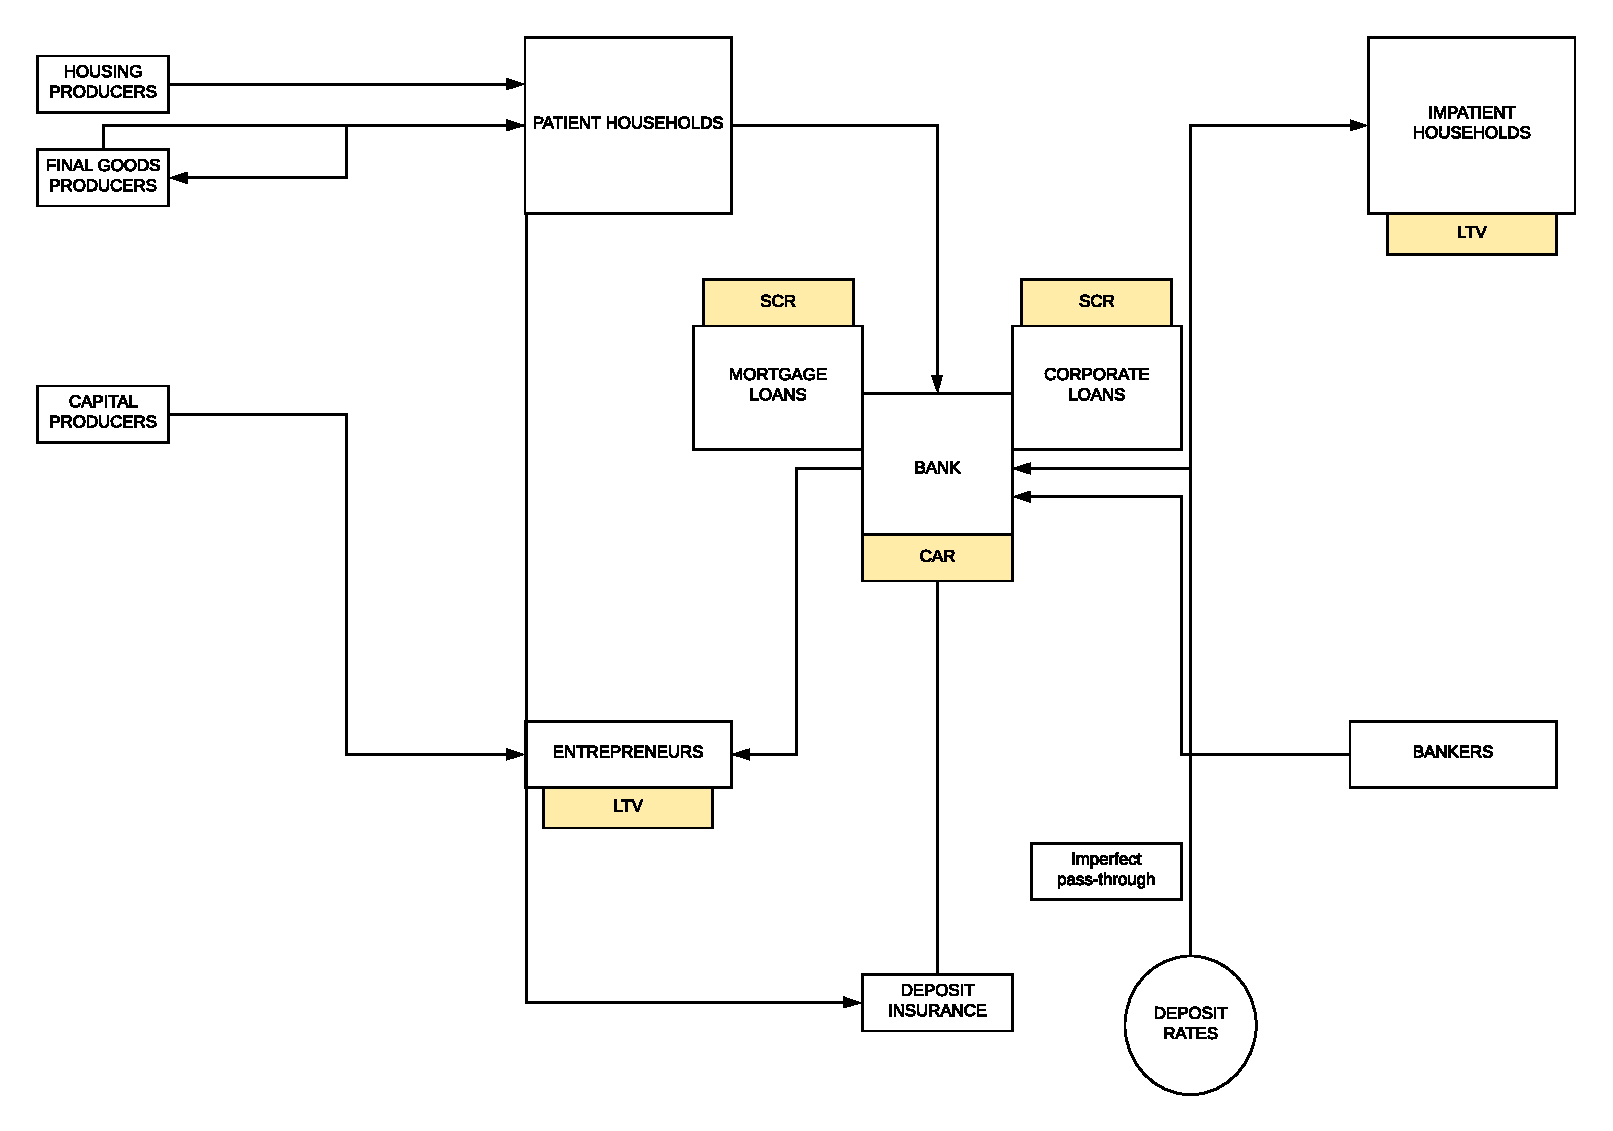
\includegraphics[scale=0.45]{3d_flowchart_prud.pdf}
%\end{figure}

%\end{frame}

\begin{frame}{Model Overview}

\begin{figure}
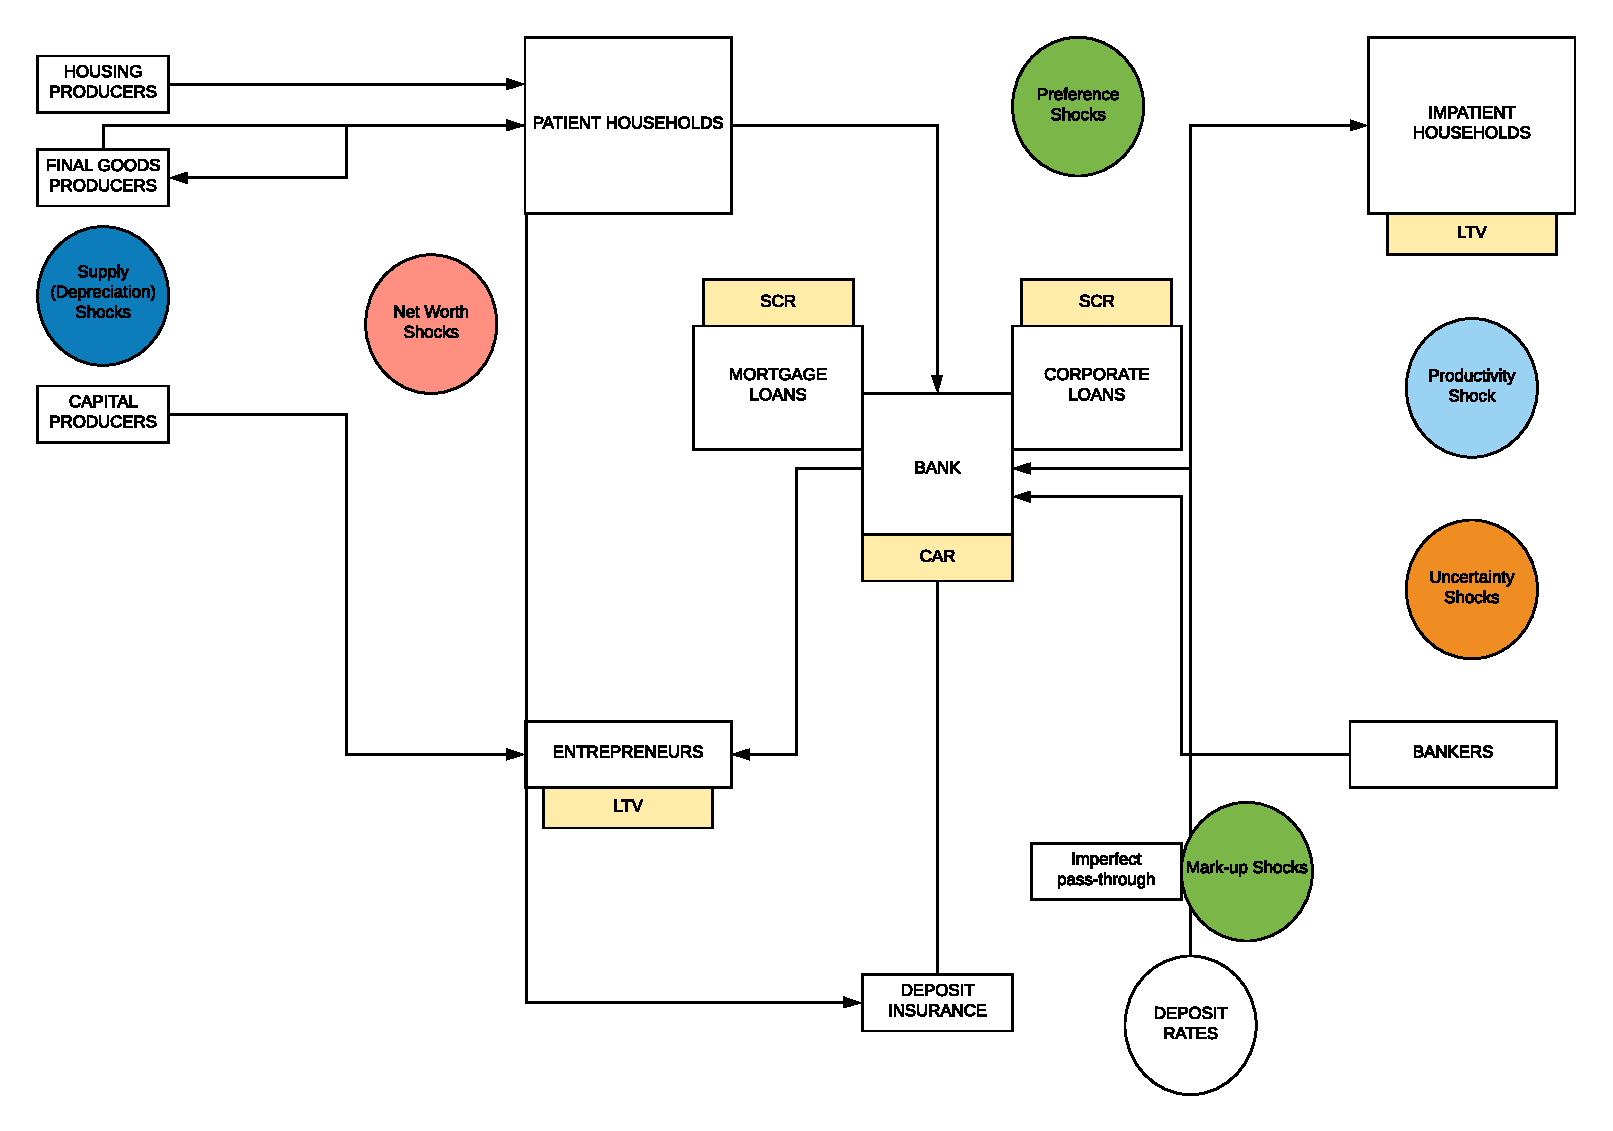
\includegraphics[scale=0.45]{3d_flowchart_full.pdf}
\end{figure}

\end{frame}



\begin{frame}{Estimation-I}


\begin{itemize}

\item Quarterly data for the U.K. economy over 1998Q1-2016Q4. 
\vspace{5 mm}
\item 10 observables in: 
\vspace{5 mm}
\begin{itemize}
\item Interest rates (Official bank rate, mortgage \& corporate rates)
\vspace{3 mm}
\item Real growth rates (output, investment, consumption and wages)
\vspace{3 mm}
\item Credit growth rates (mortgage \& corporate sectors) 
\vspace{3 mm}
\item House price growth
\end{itemize}

\vspace{5 mm}
\item Model (partially) estimated using Bayesian likelihood methods. 
\end{itemize}



\end{frame}





\begin{frame}{Estimation-II}

\begin{figure}[H]
\centering
\caption{{Example: estimated interest-rate pass through}}
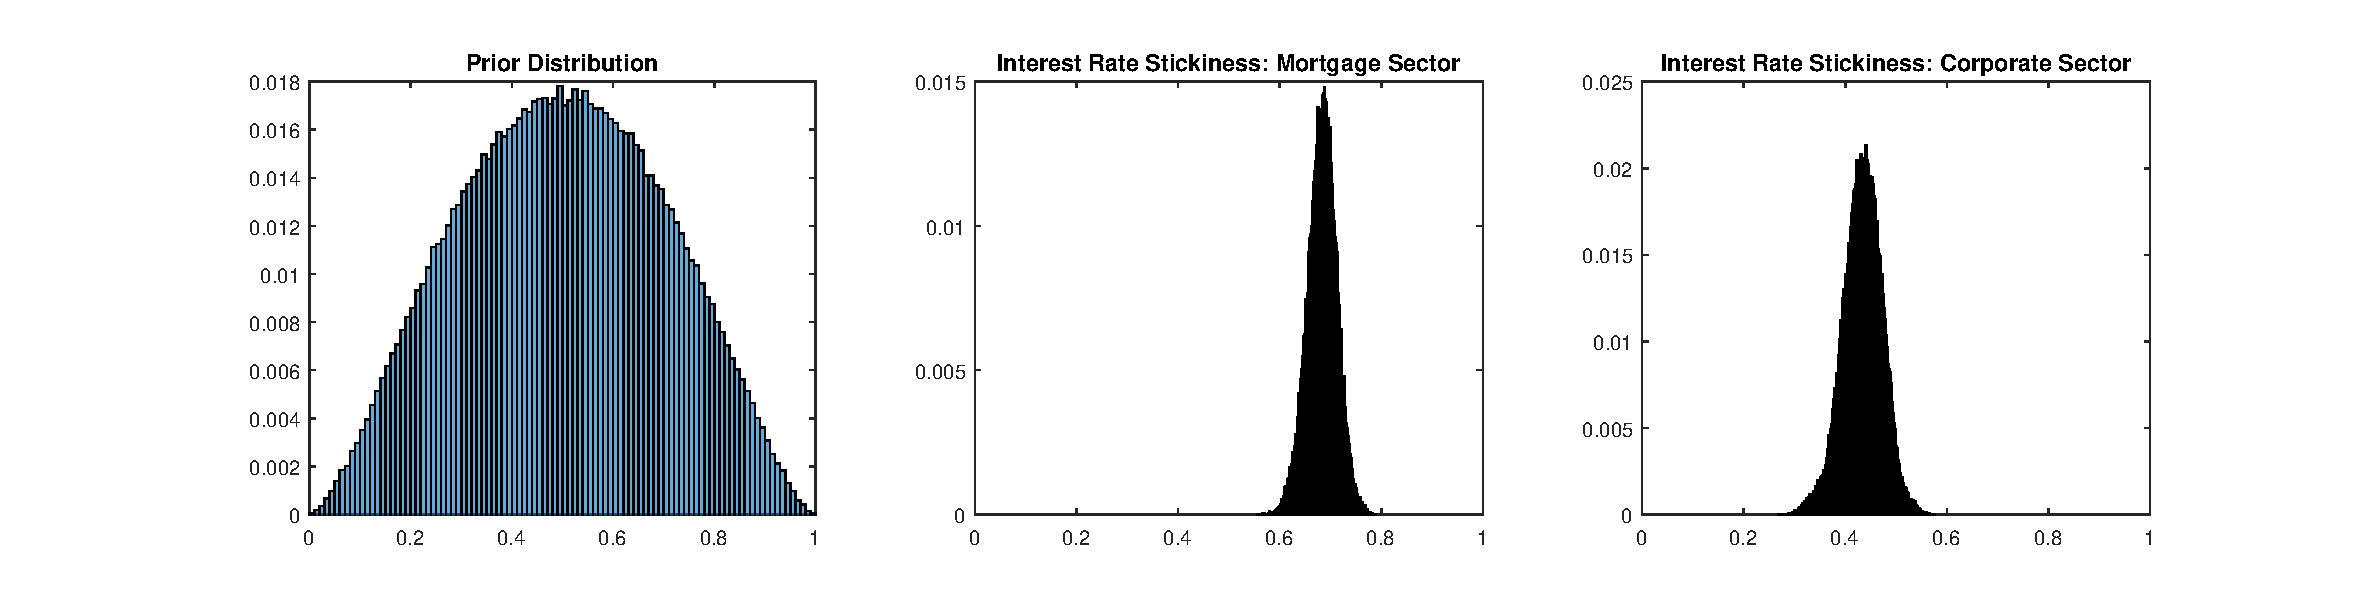
\includegraphics[scale=0.4]{posteriordistributions_calvo2.pdf}
\end{figure}


\begin{itemize}
\item Average Bank Rate pass-through is $[4.73,5.93]$ months on corporate rates and $[8.21,11.1]$ months on mortgage rates.

\end{itemize}

\end{frame}


\begin{frame}{Estimated shocks over 1998Q1-2016Q4.}
%\begin{itemize}
%\item What does it take in the model to generate the observed data? 

\begin{itemize}
\item Sequence of shocks over the estimation sample. 
%\end{itemize}

\end{itemize}
\begin{figure}[H]
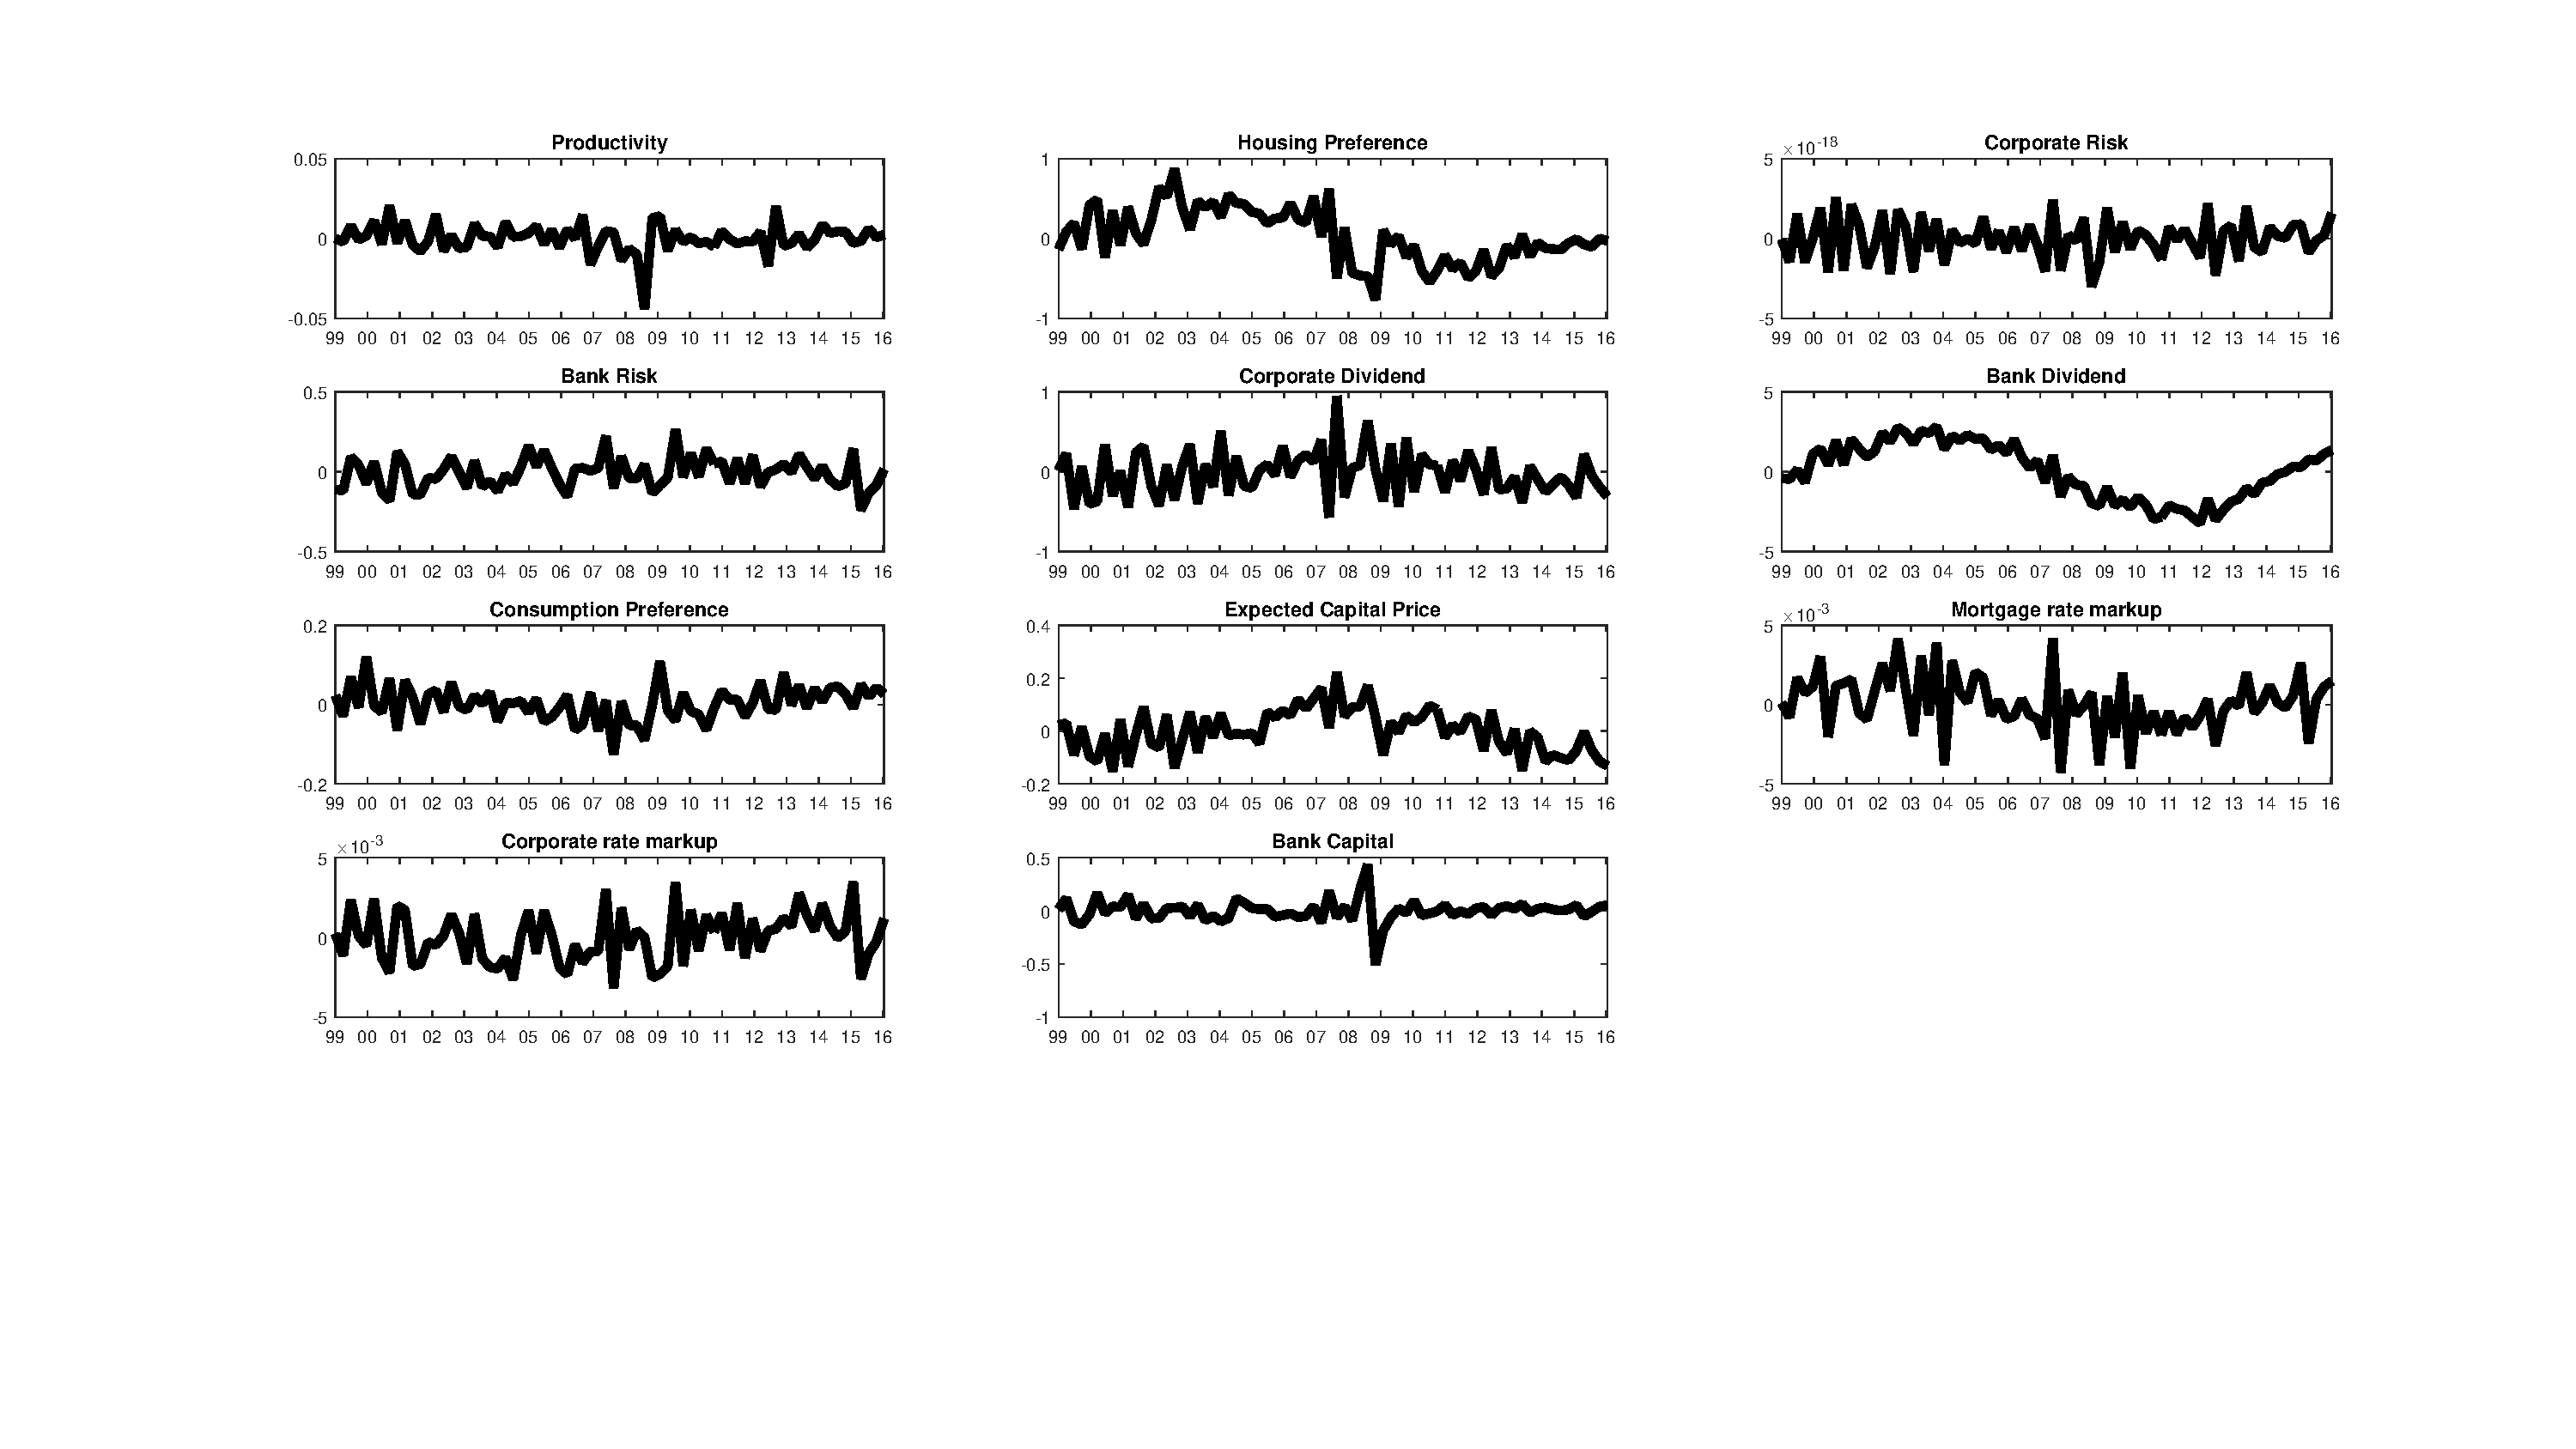
\includegraphics[scale=0.3]{smoothed_shocks.pdf}
\end{figure}

\end{frame}



\begin{frame}{Historical Variance Decompositions: Output   Growth }

%\begin{itemize}

%\item Each variable over the sample is a combination of shocks
%\end{itemize}

\begin{figure}
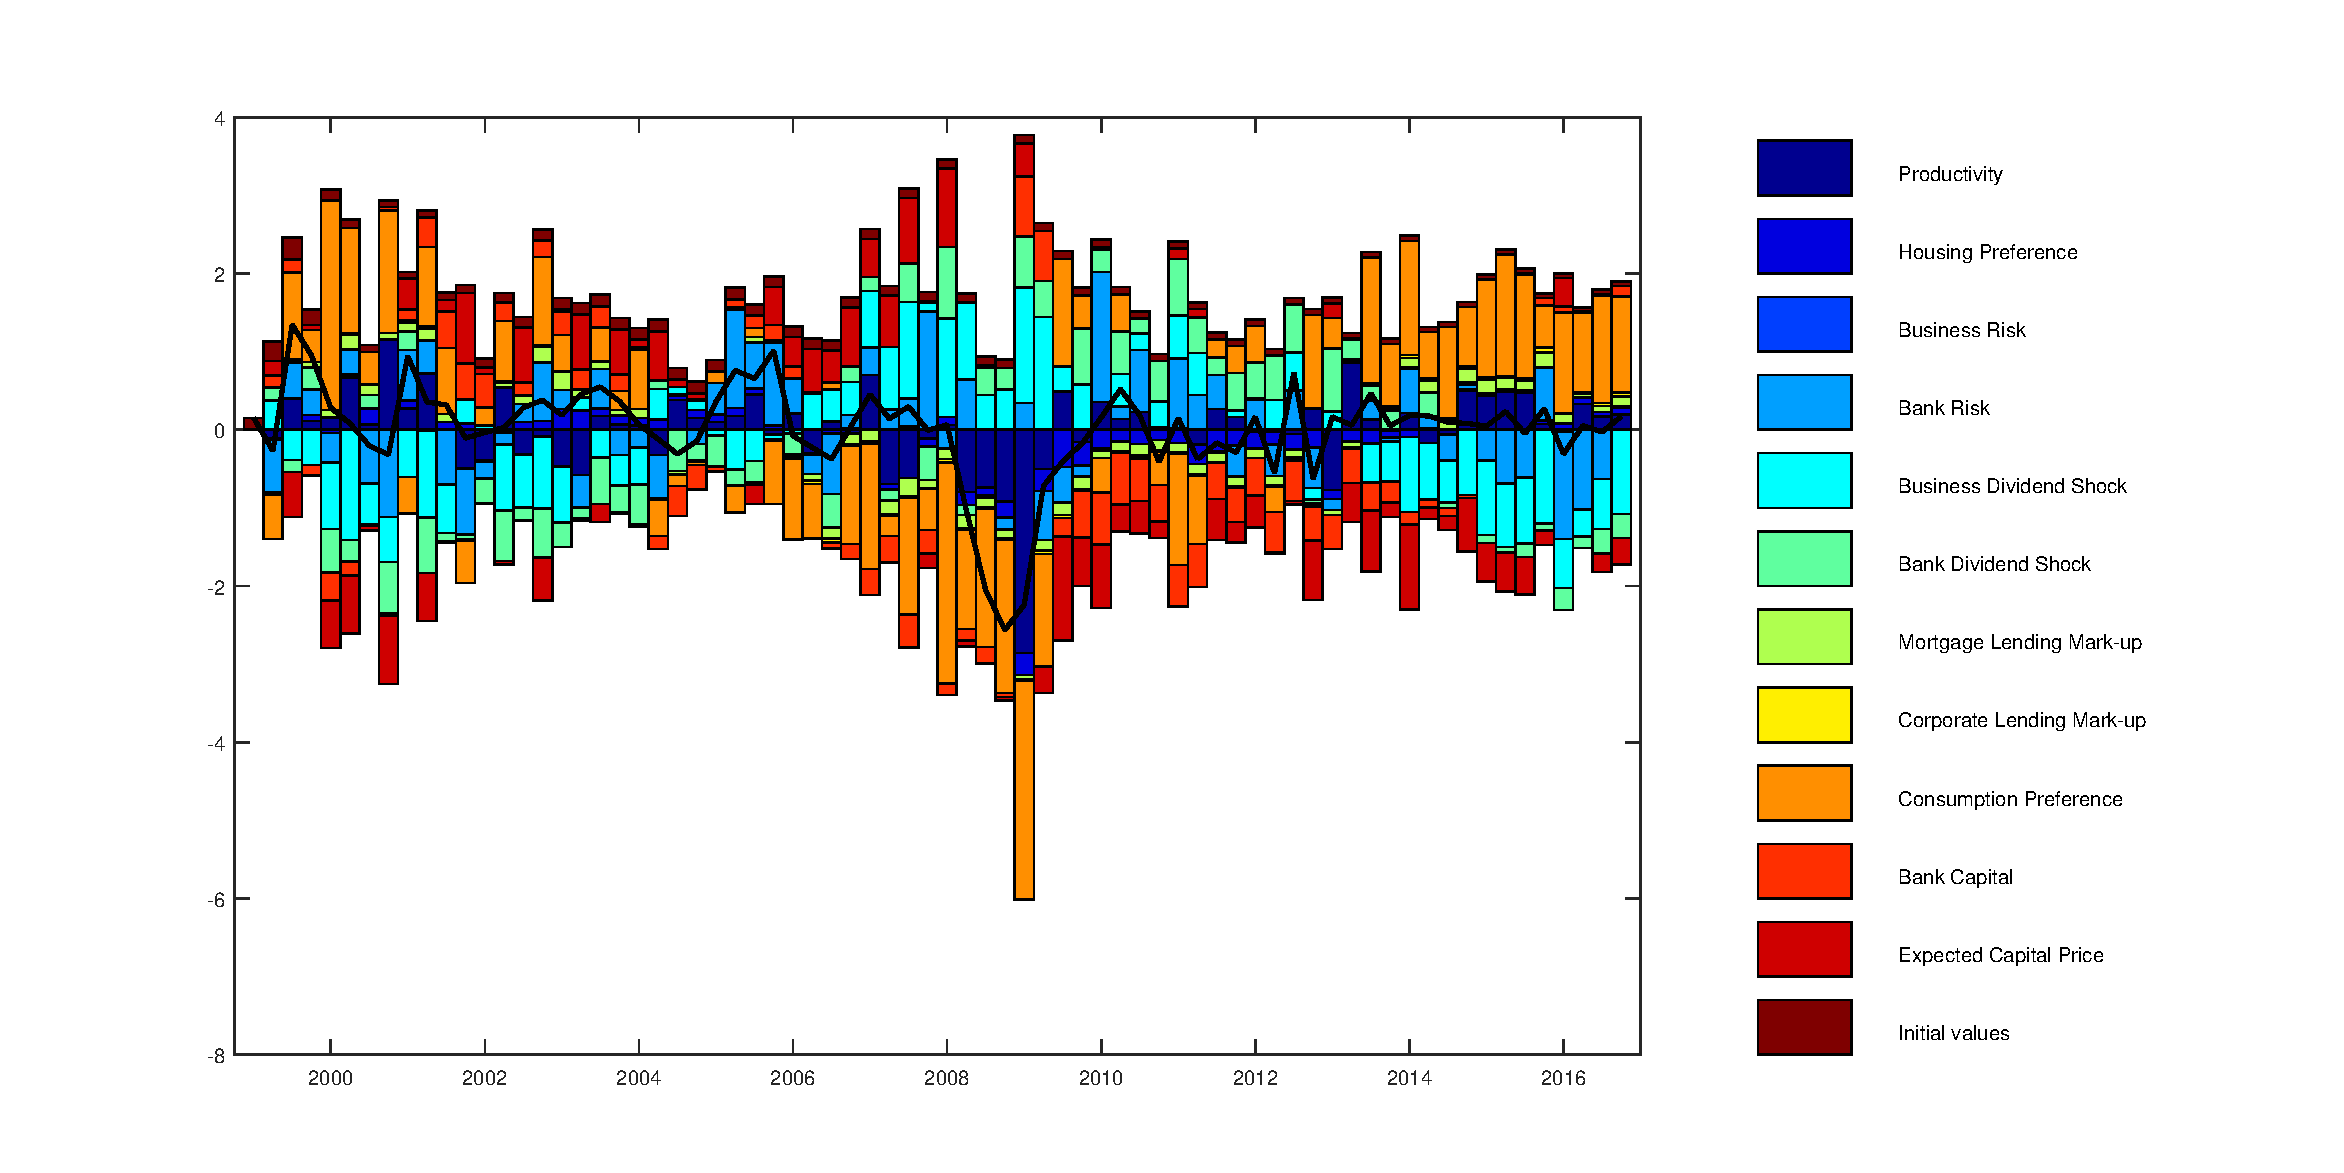
\includegraphics[scale=0.36]{decomp_dy.pdf}
\end{figure}
\end{frame}




\begin{frame}{Historical Variance Decomposition: Household Lending Growth }

\begin{figure}
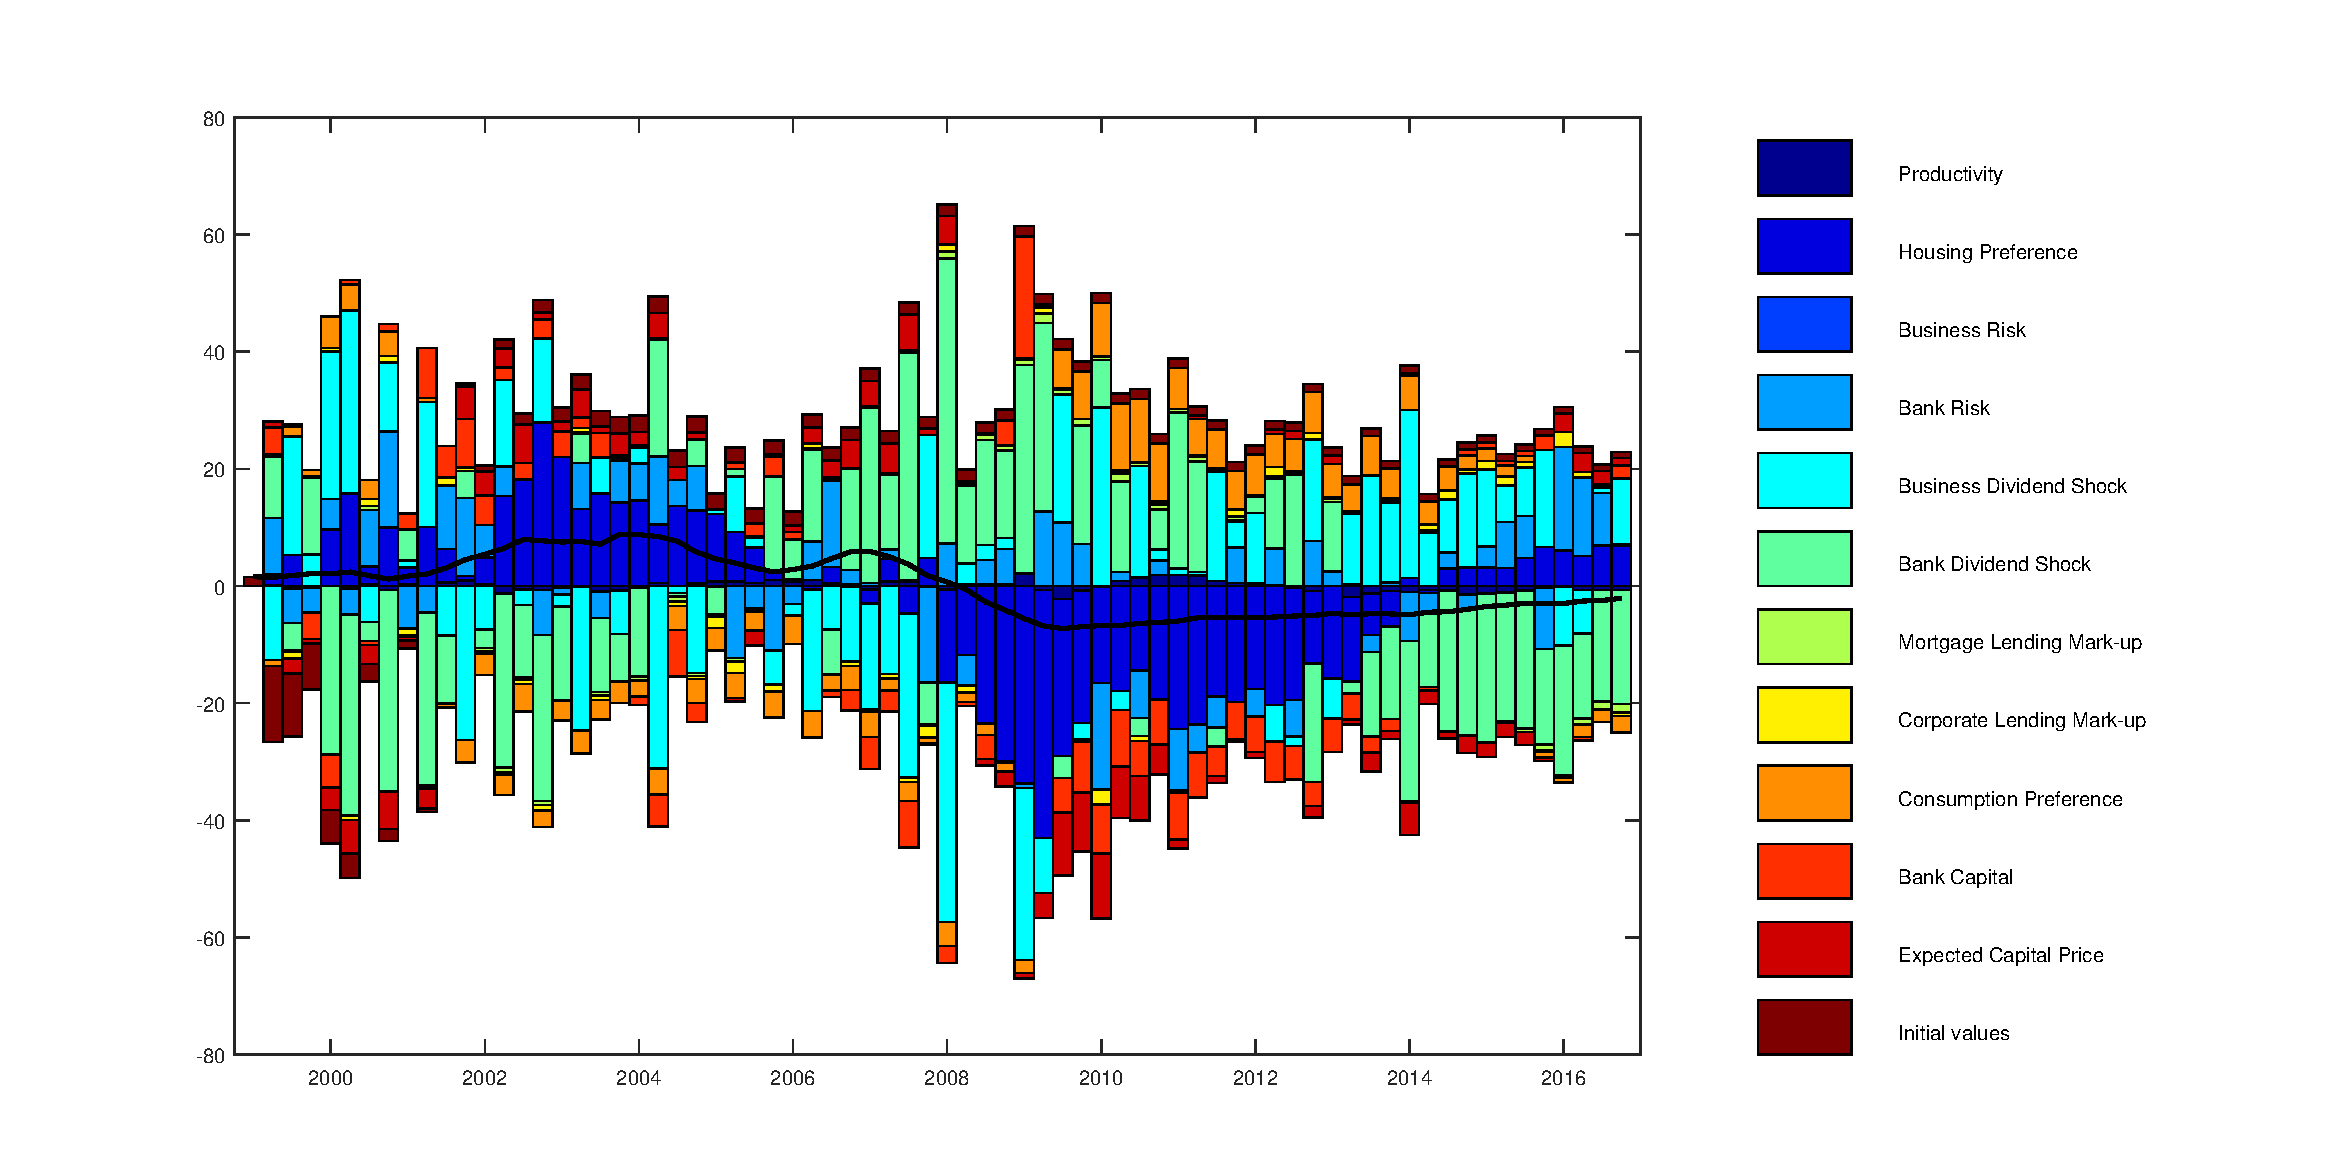
\includegraphics[scale=0.36]{decomp_dbm.pdf}
\end{figure}
\end{frame}



\begin{frame}{Historical Variance Decomposition: Corporate Lending Growth }

\begin{figure}
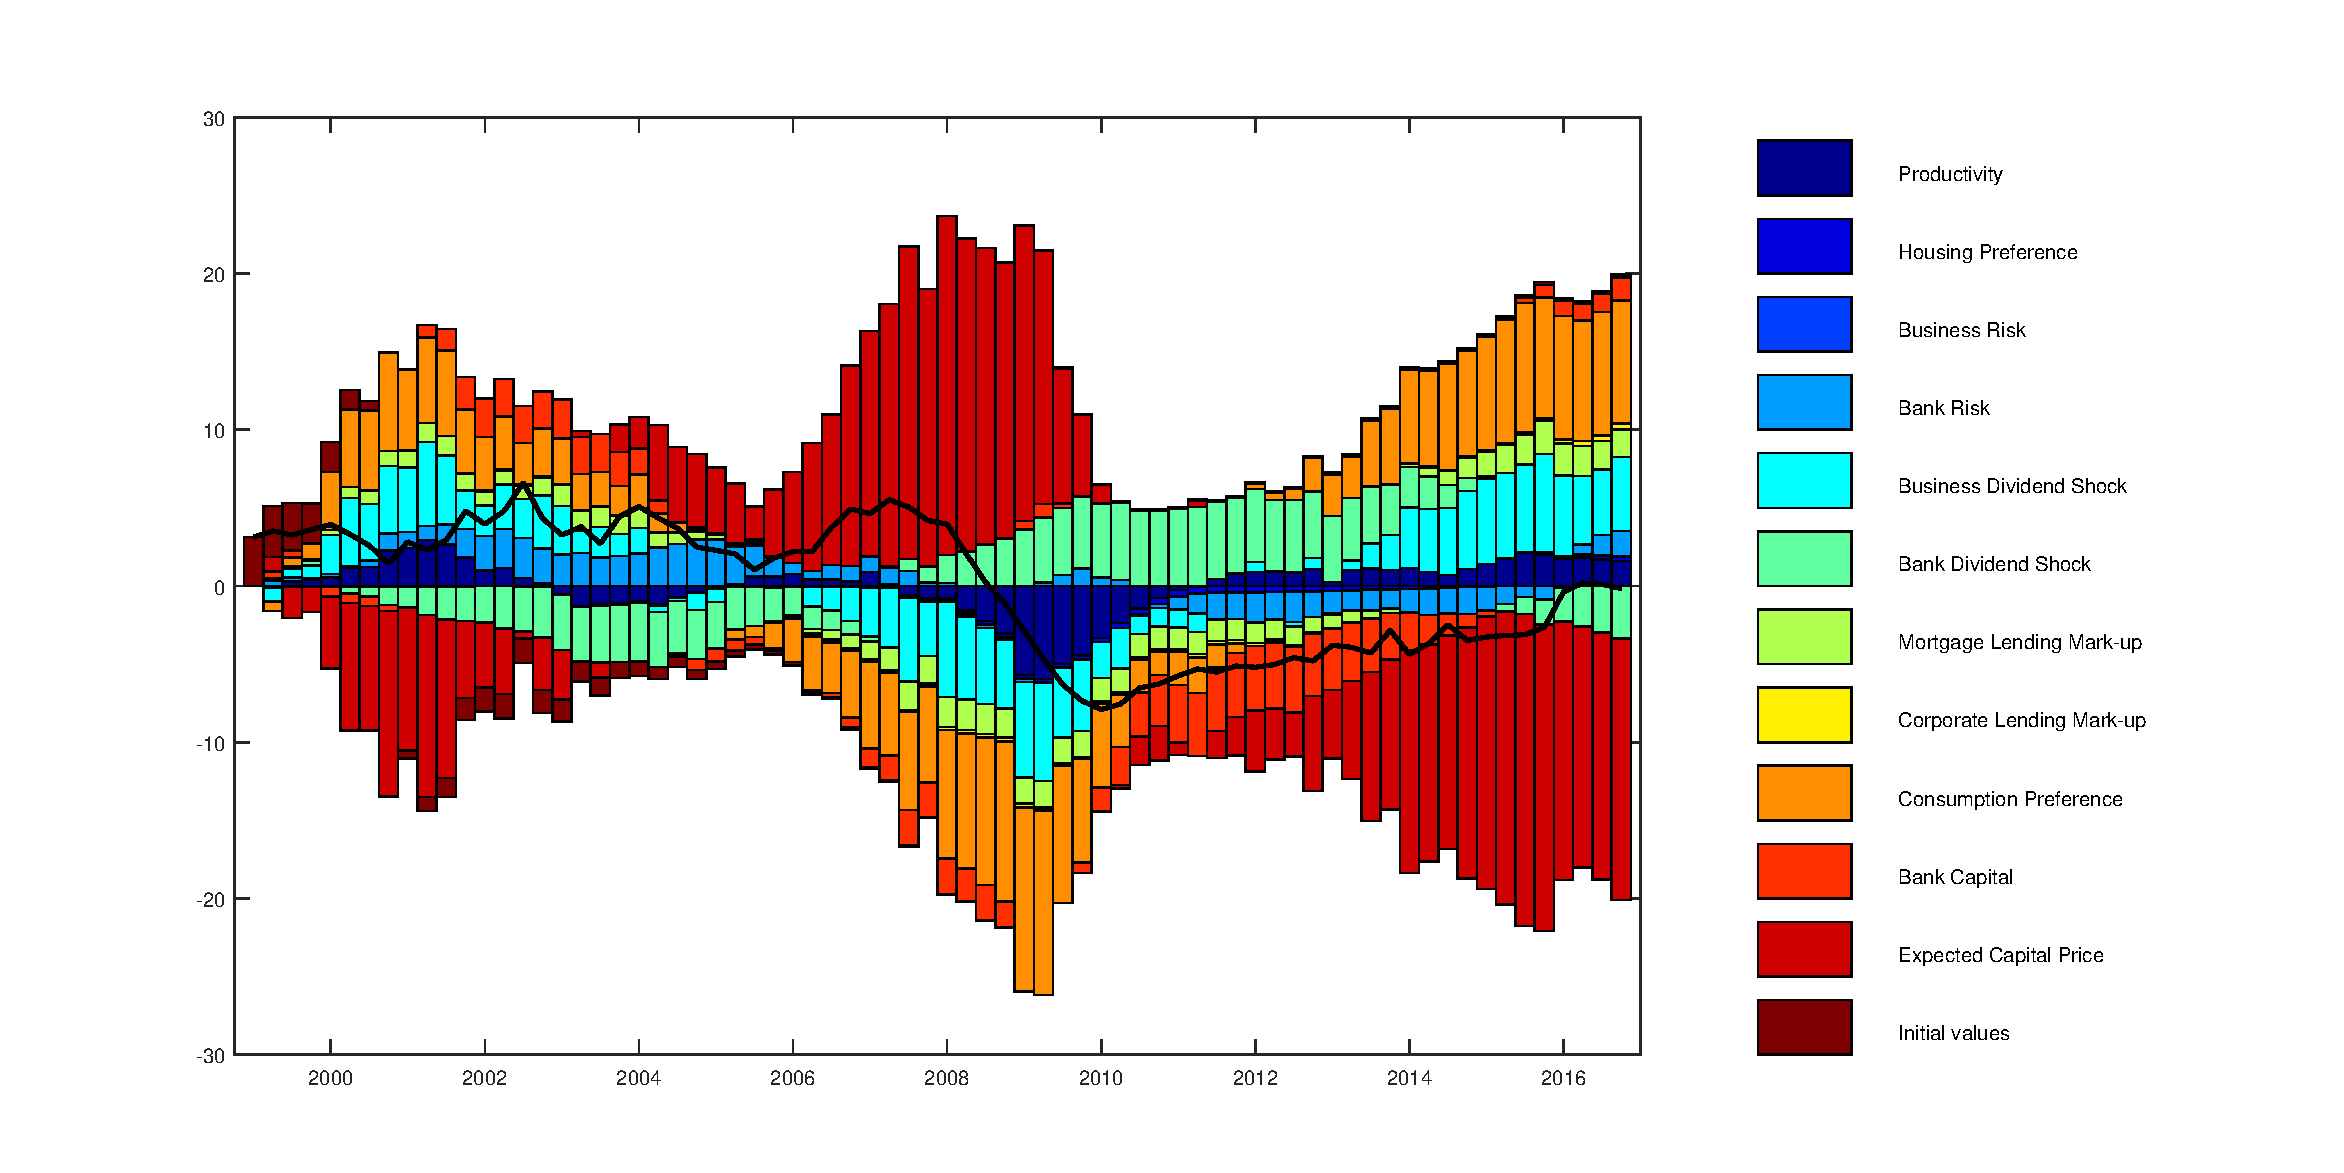
\includegraphics[scale=0.36]{decomp_dbe.pdf}
\end{figure}
\end{frame}


\begin{frame}{Historical Variance Decomposition: Consumption Growth }

\begin{figure}
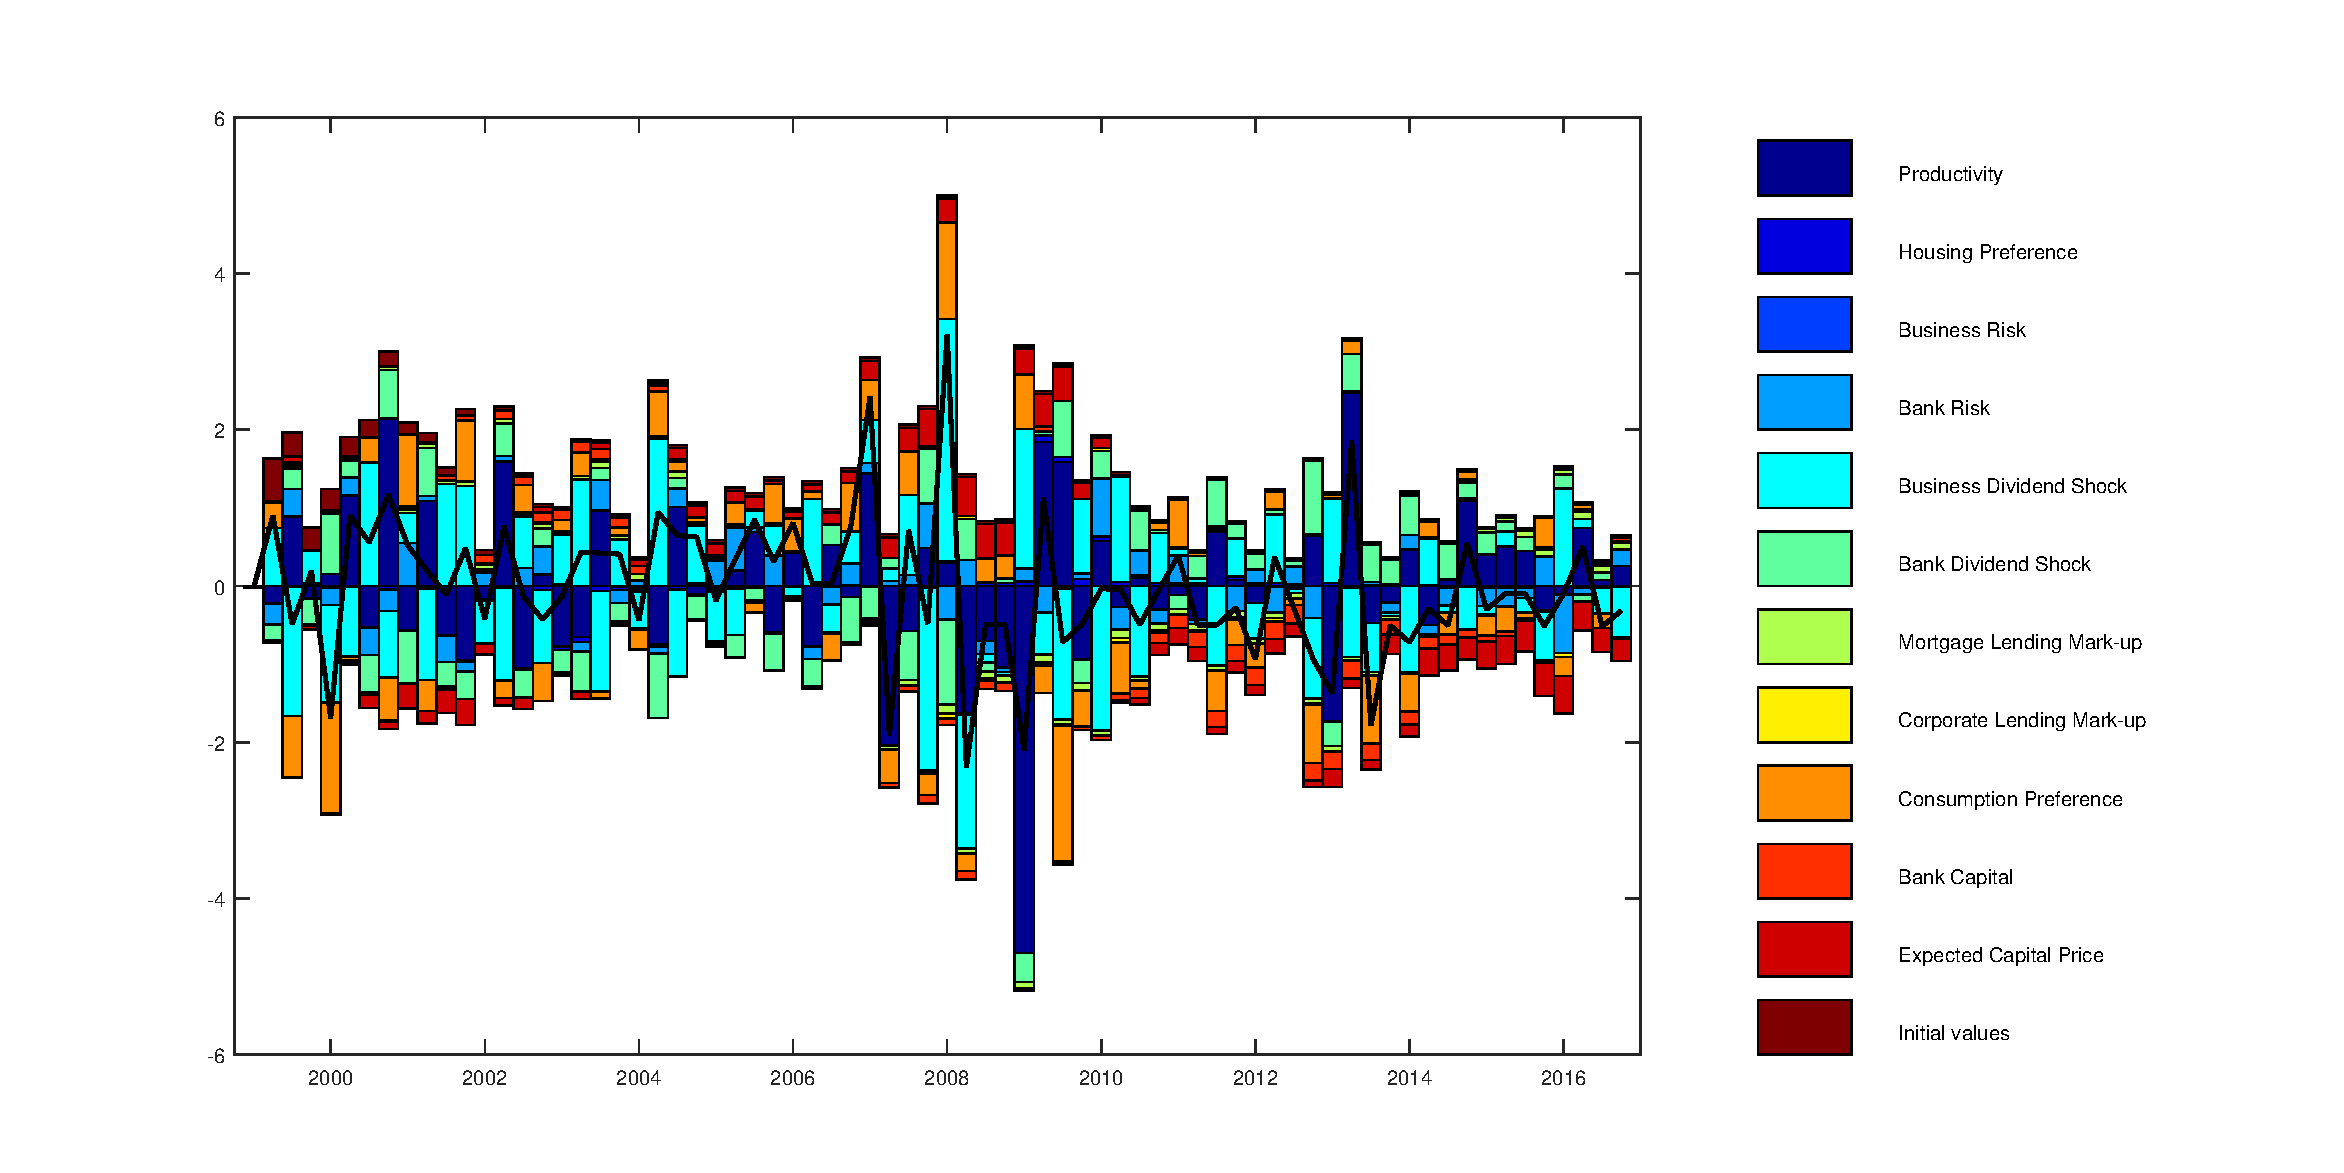
\includegraphics[scale=0.36]{decomp_dc.pdf}
\end{figure}
\end{frame}



\begin{frame}{Historical Variance Decomposition: Investment Growth }

\begin{figure}
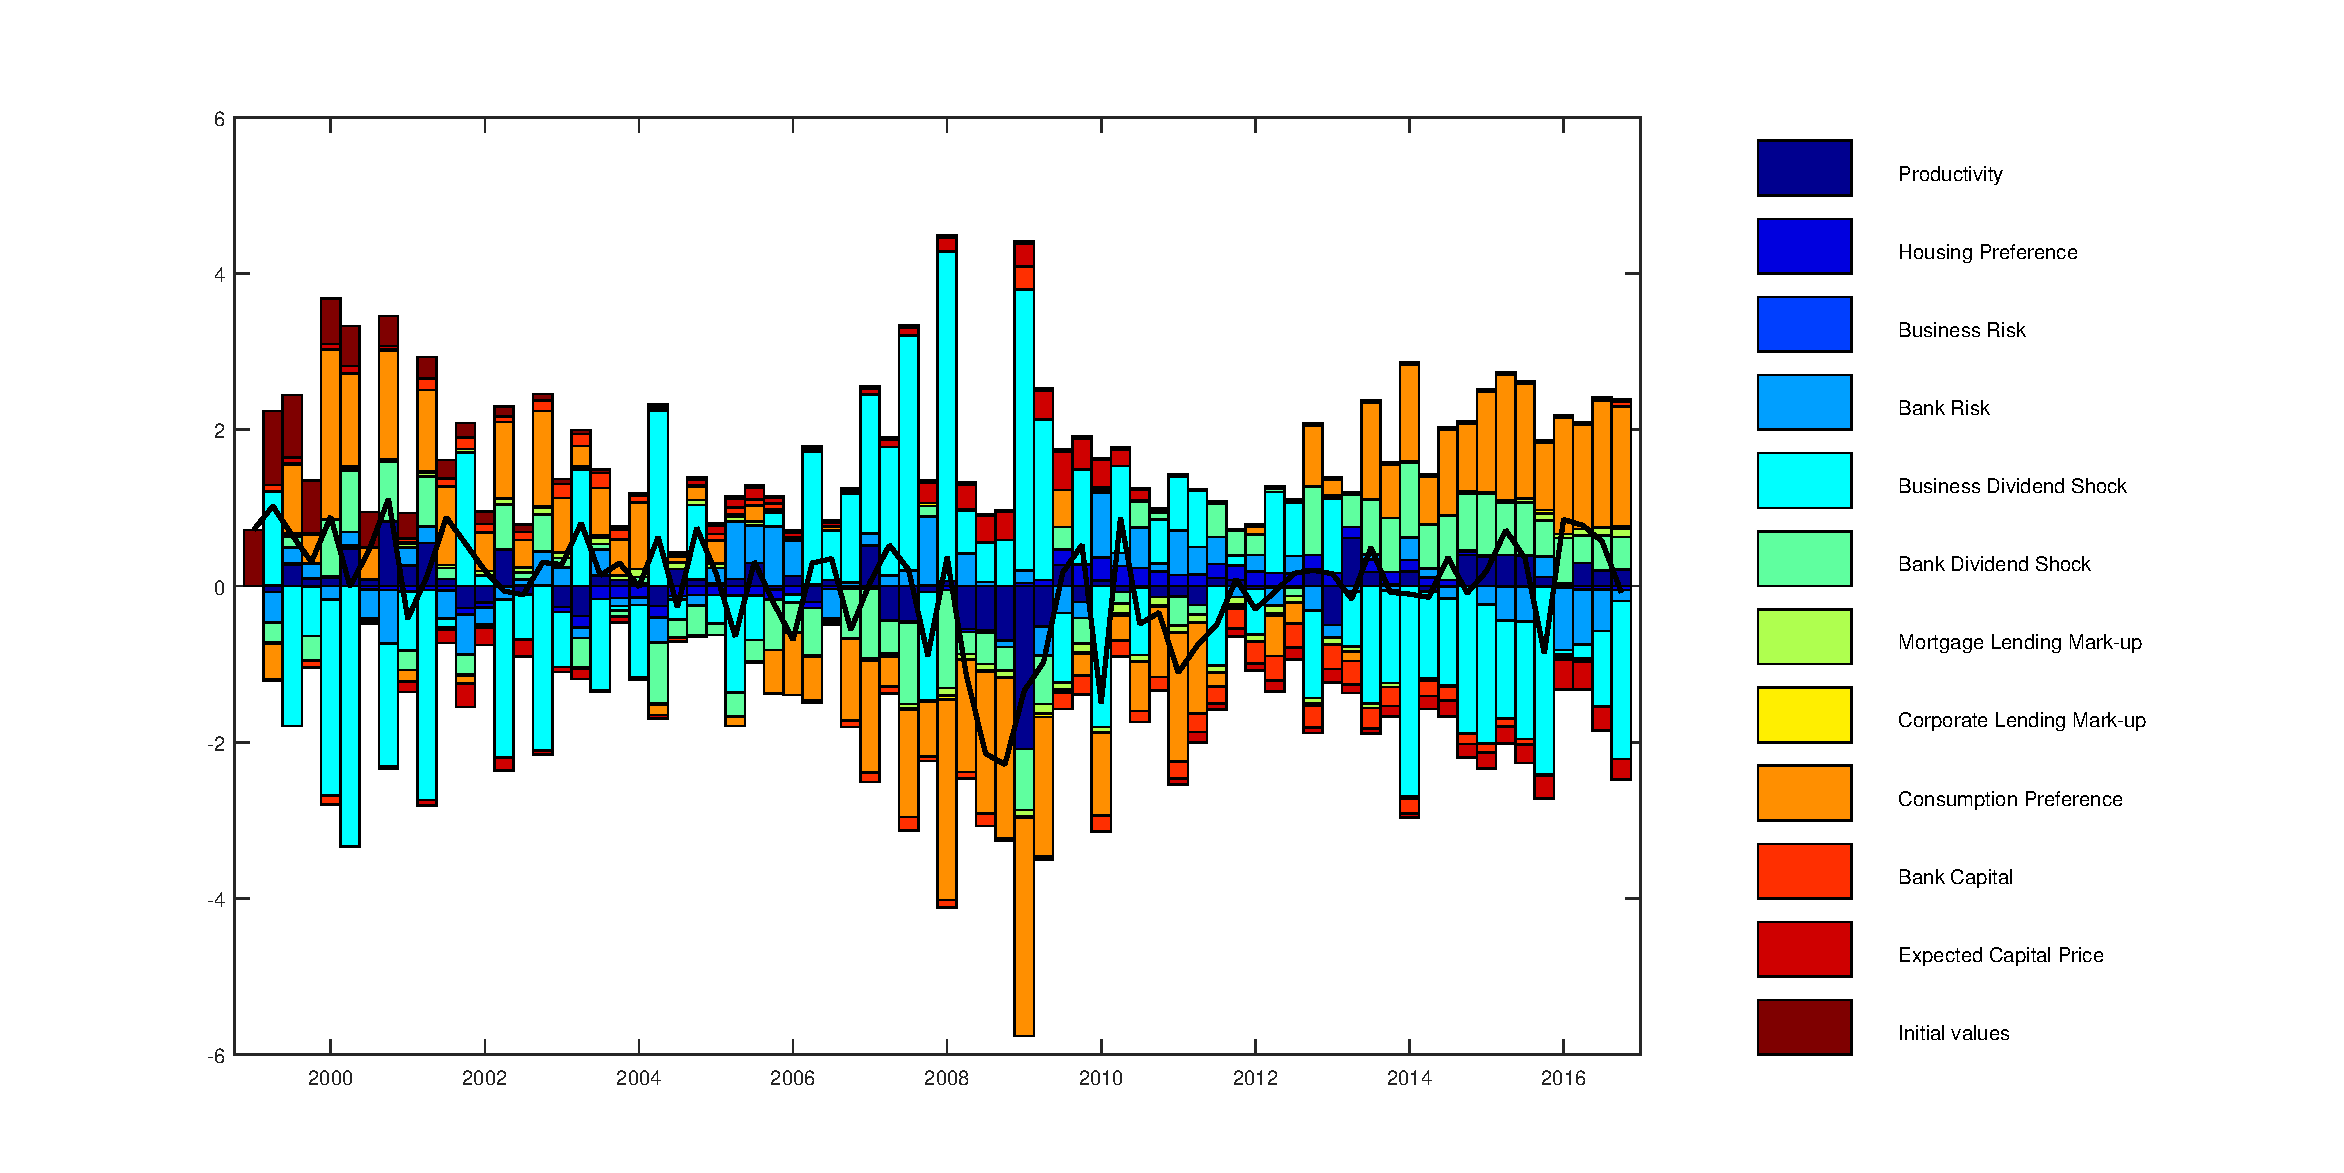
\includegraphics[scale=0.36]{decomp_dinve.pdf}
\end{figure}
\end{frame}



\begin{frame}{Historical Variance Decomposition: House Price Growth }

\begin{figure}
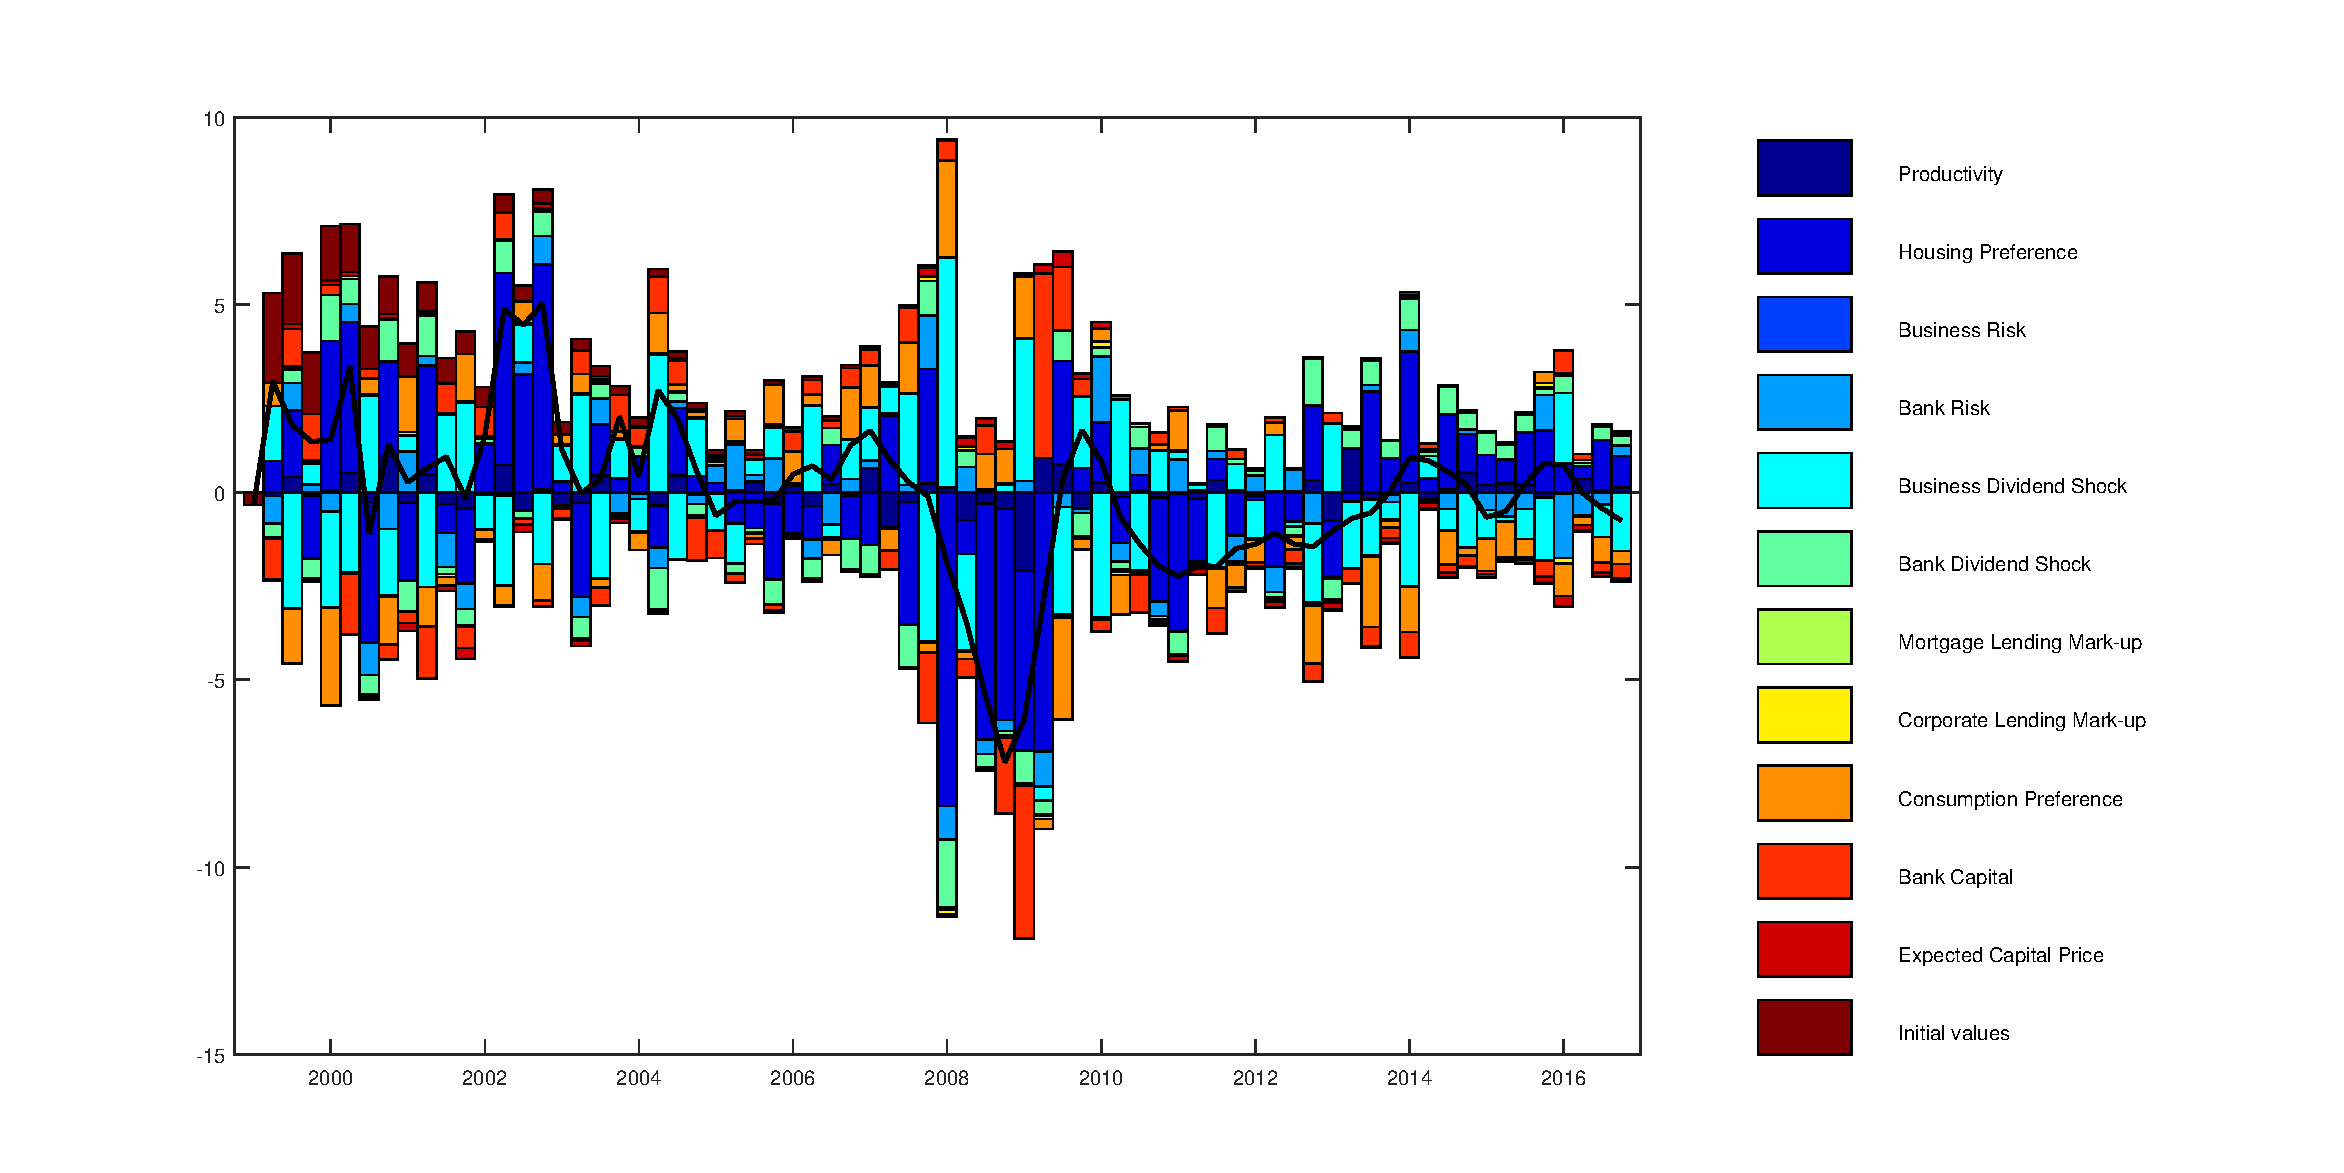
\includegraphics[scale=0.36]{decomp_dqh.pdf}
\end{figure}
\end{frame}


\begin{frame}{Historical Variance Decomposition: Wage Growth }

\begin{figure}
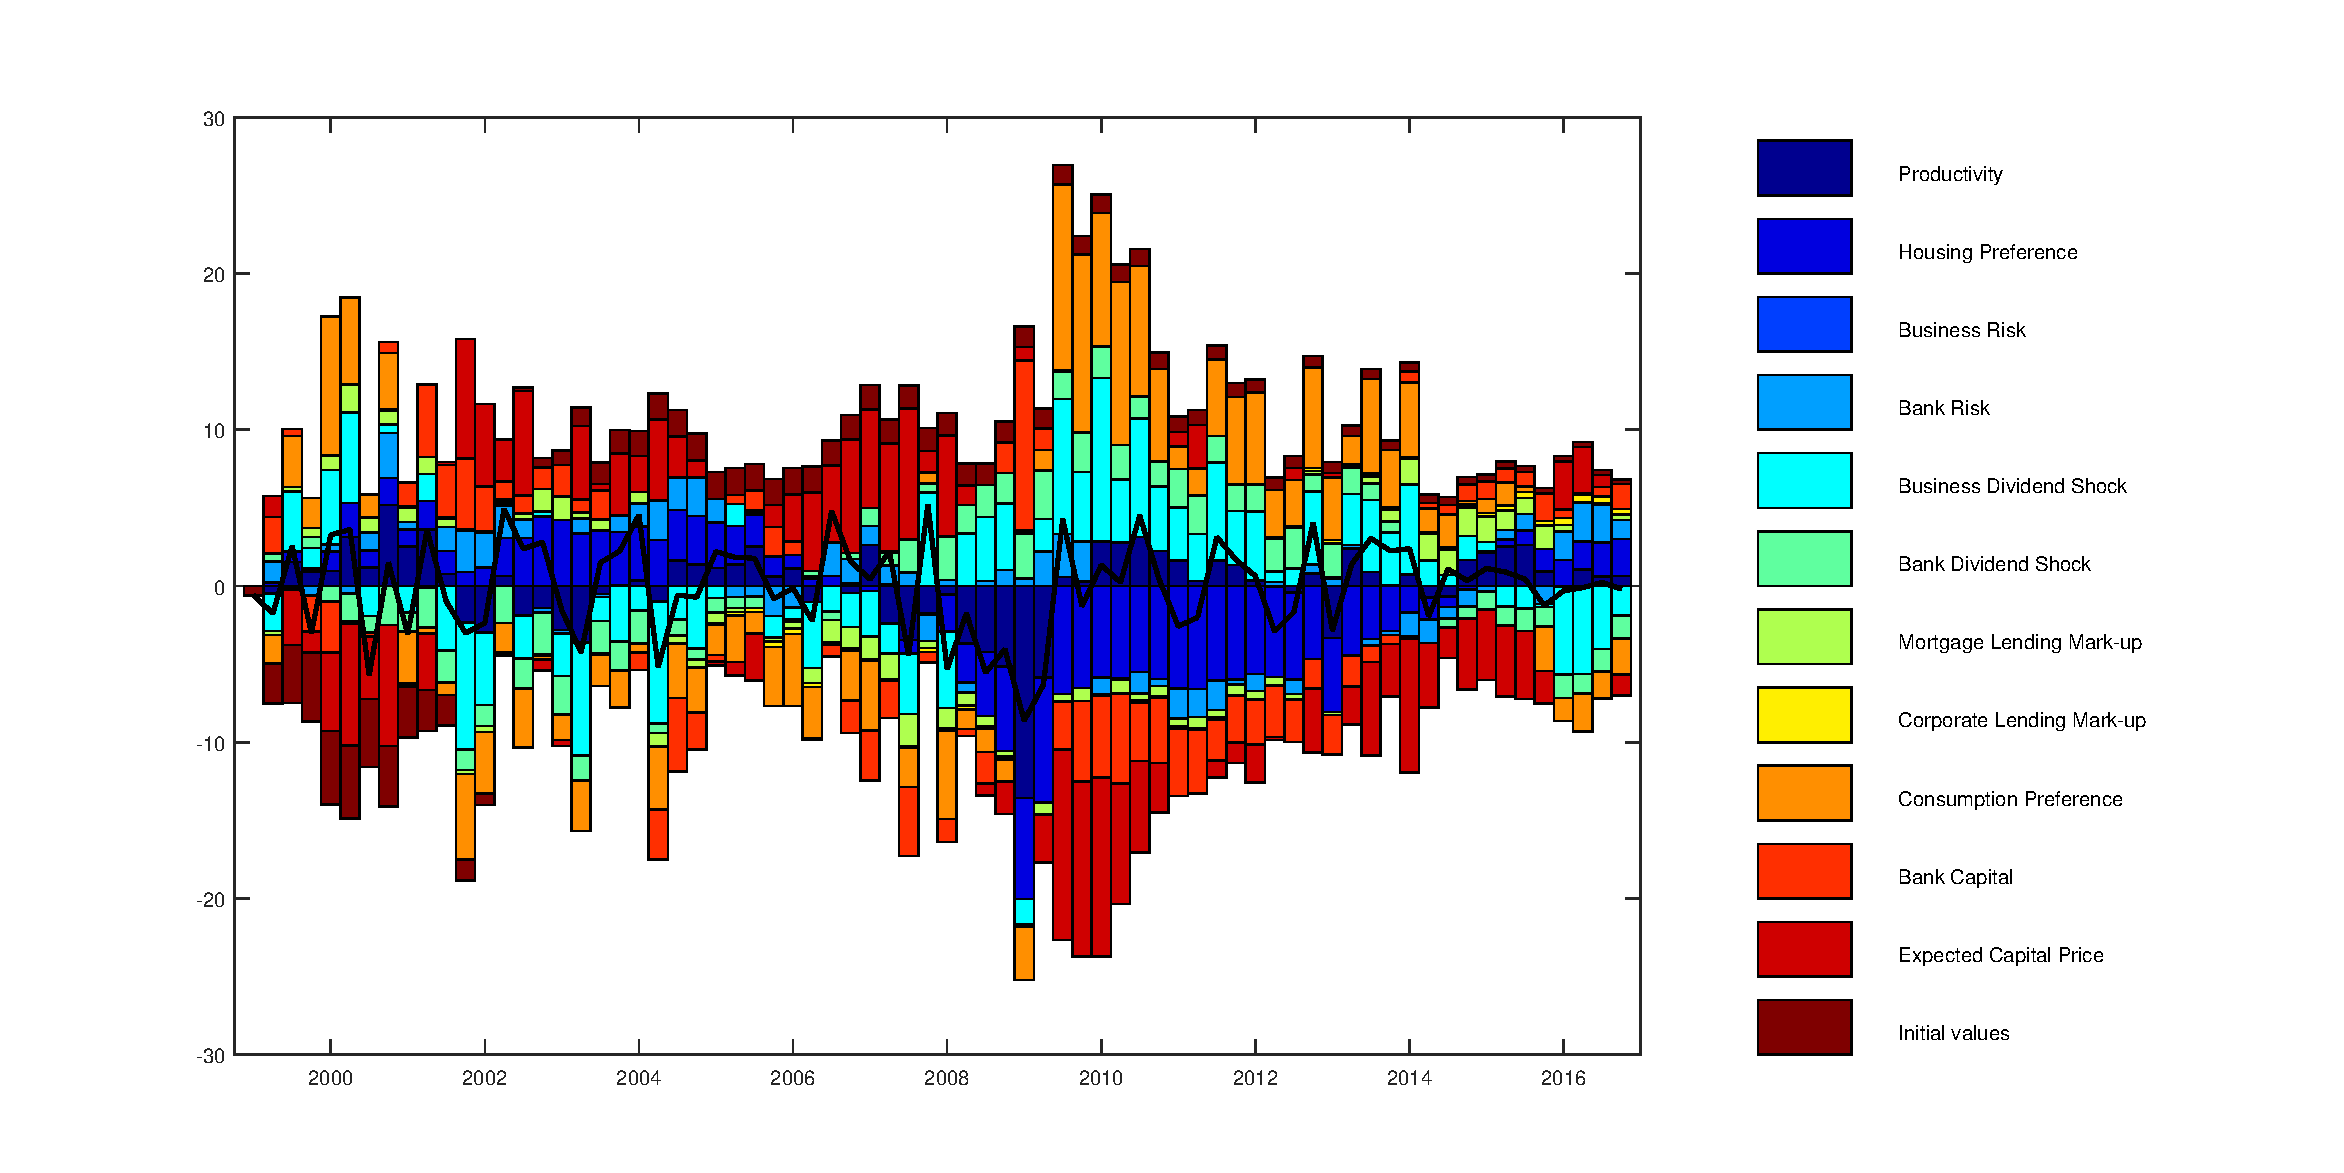
\includegraphics[scale=0.36]{decomp_dw.pdf}
\end{figure}
\end{frame}



\begin{comment}

\begin{frame}{Some key unobservables estimated by the model}

\begin{itemize}
\item Household defaults are dominant during the crisis period.
\item Welfare of both household types have an upward trend before the crisis, and downward afterwards.

\end{itemize}    

\begin{figure}
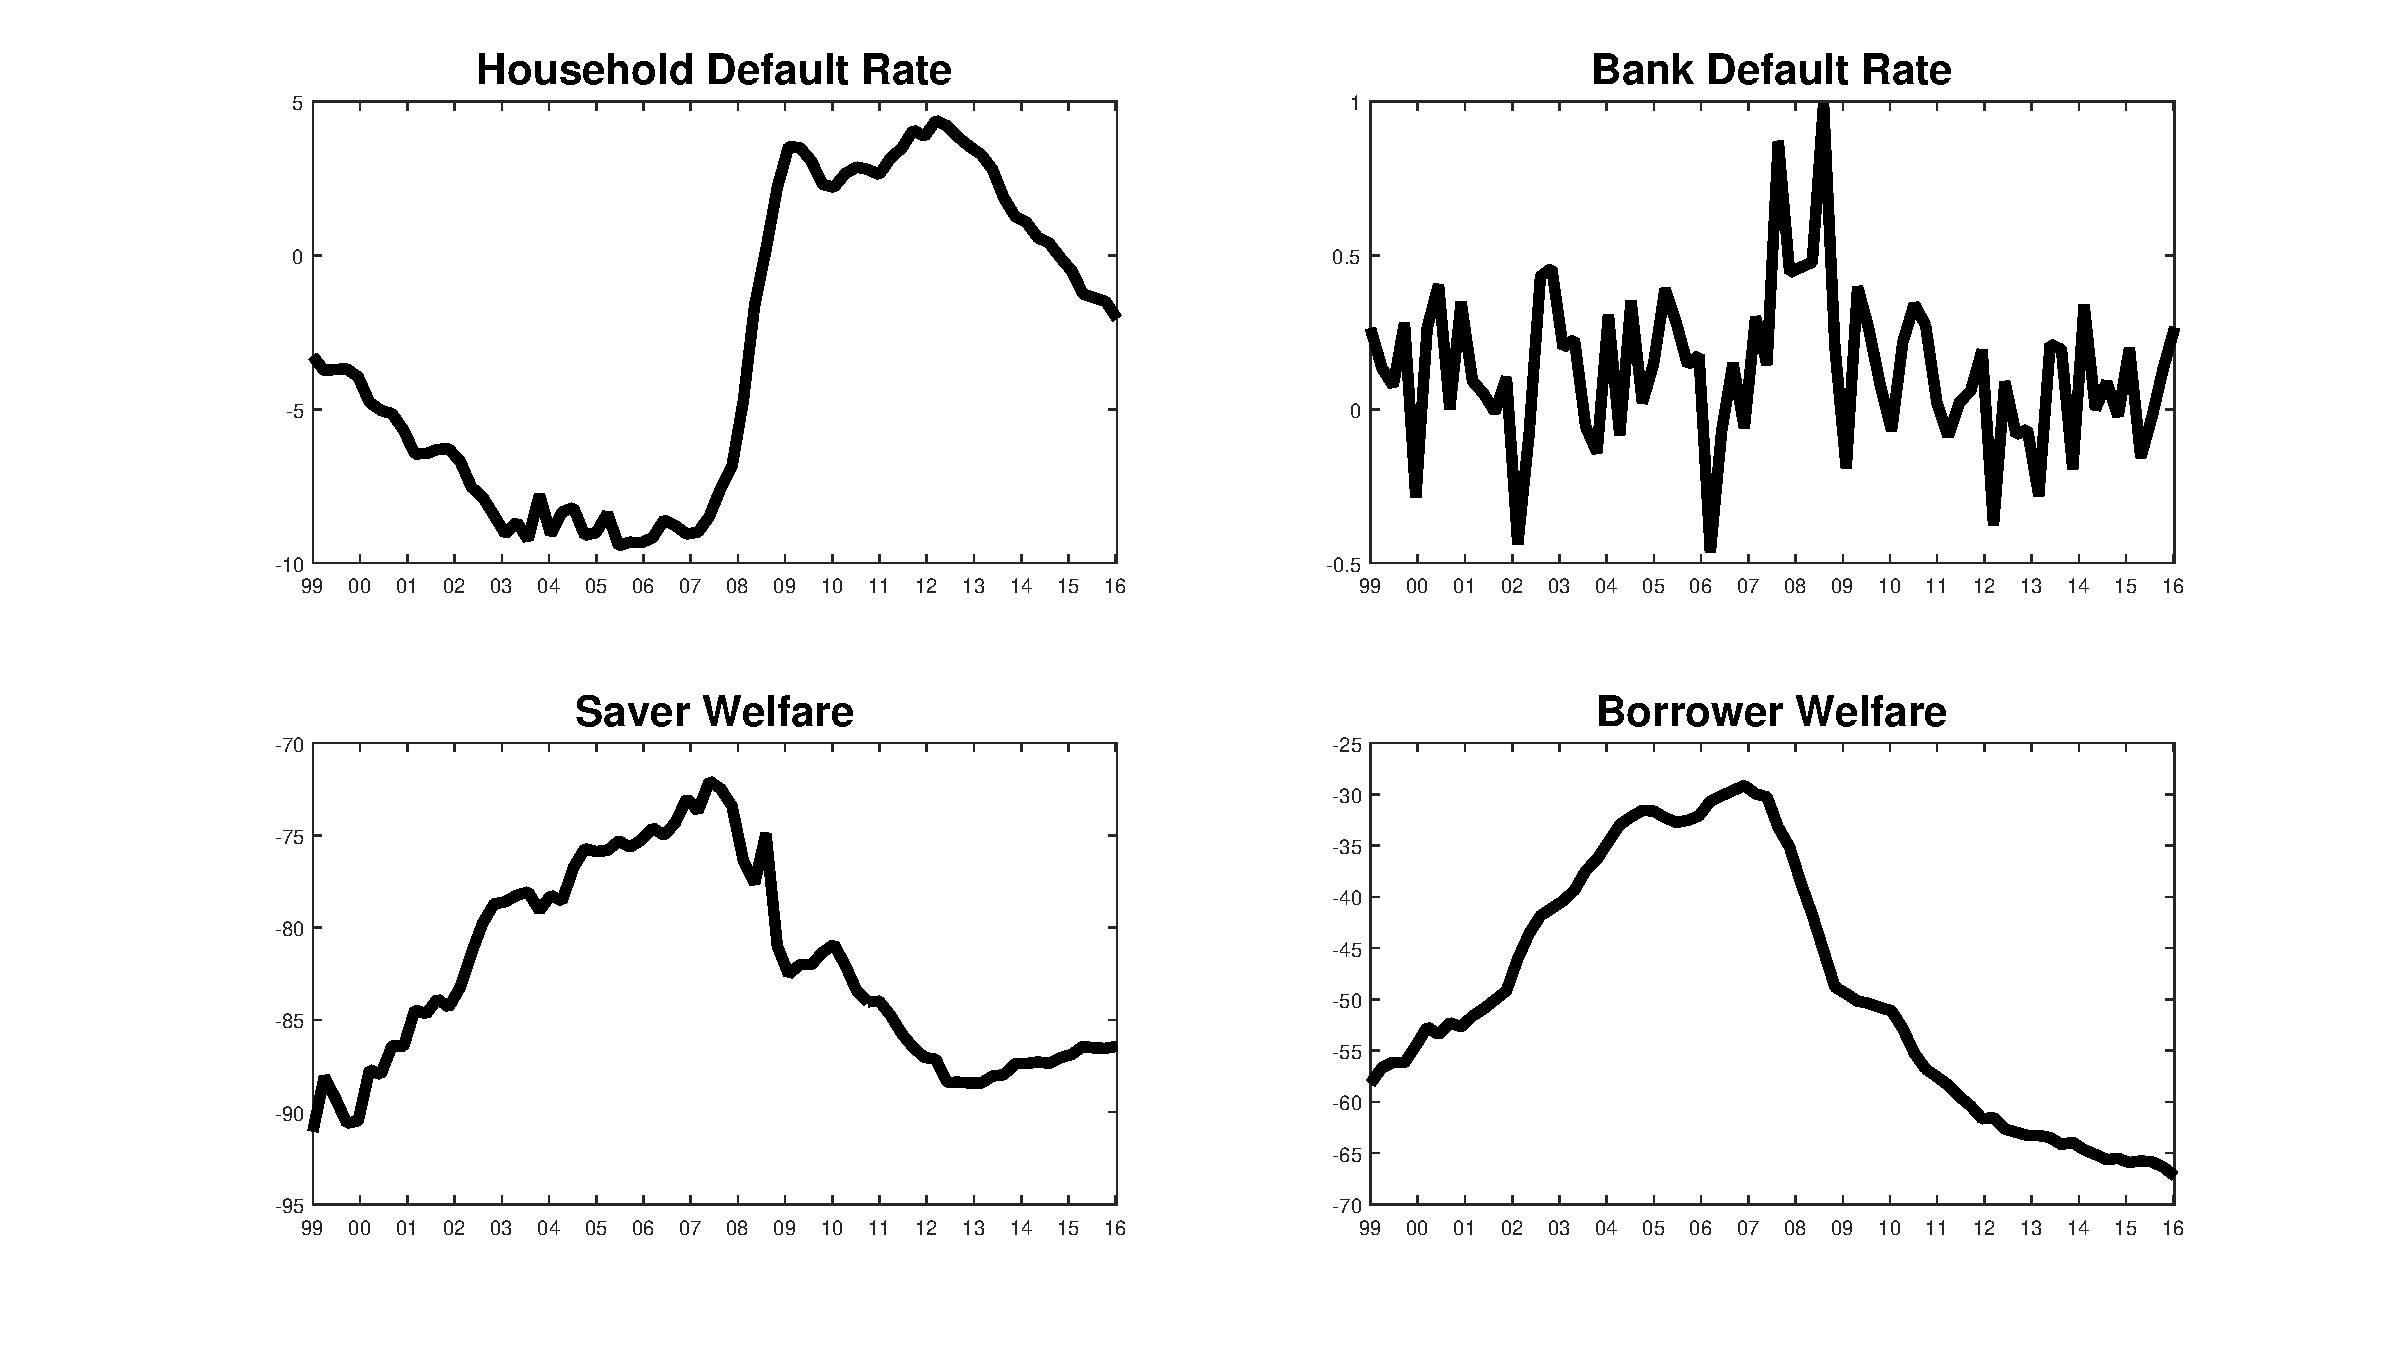
\includegraphics[scale=0.25]{smoothed_variables.pdf}
\end{figure}


\end{frame}



\begin{frame}{Macroprudential Policy}

\begin{itemize}

\item Available tools in the model: 
\vspace{3 mm}
\begin{itemize}
\item Minimum and sectoral capital requirements (Benchmark: 11 \% CAR, no SCR)
\vspace{3 mm}
\item LTV limit on businesses and households (Benchmark: 86 \%)
\vspace{3 mm}
\item CCyB (Benchmark: 0)
\end{itemize}

\pause 

\vspace{5 mm}
\item Steady-state welfare analysis
\vspace{5 mm}
\item Counterfactuals
\vspace{5 mm}
\item Interest rate stickiness \& Macroprudential tools interaction

\end{itemize}
\end{frame}



\begin{frame}{Example: Sectoral Capital Requirements on Mortgage Lending and Key Variables in Steady-state}

\begin{figure}[H]
\centering
%\caption{Sectoral capital requirements on mortgage lending with a baseline of 11 \%. Welfare maximizing value is 20.7 \% with a weight of 0 on volatility. It decreases to 17.6 \% with a weight of 0.1 on the volatility.
%\textbf{Welfare improvement: 7.47 \% and 4.26 \% respectively.} } 
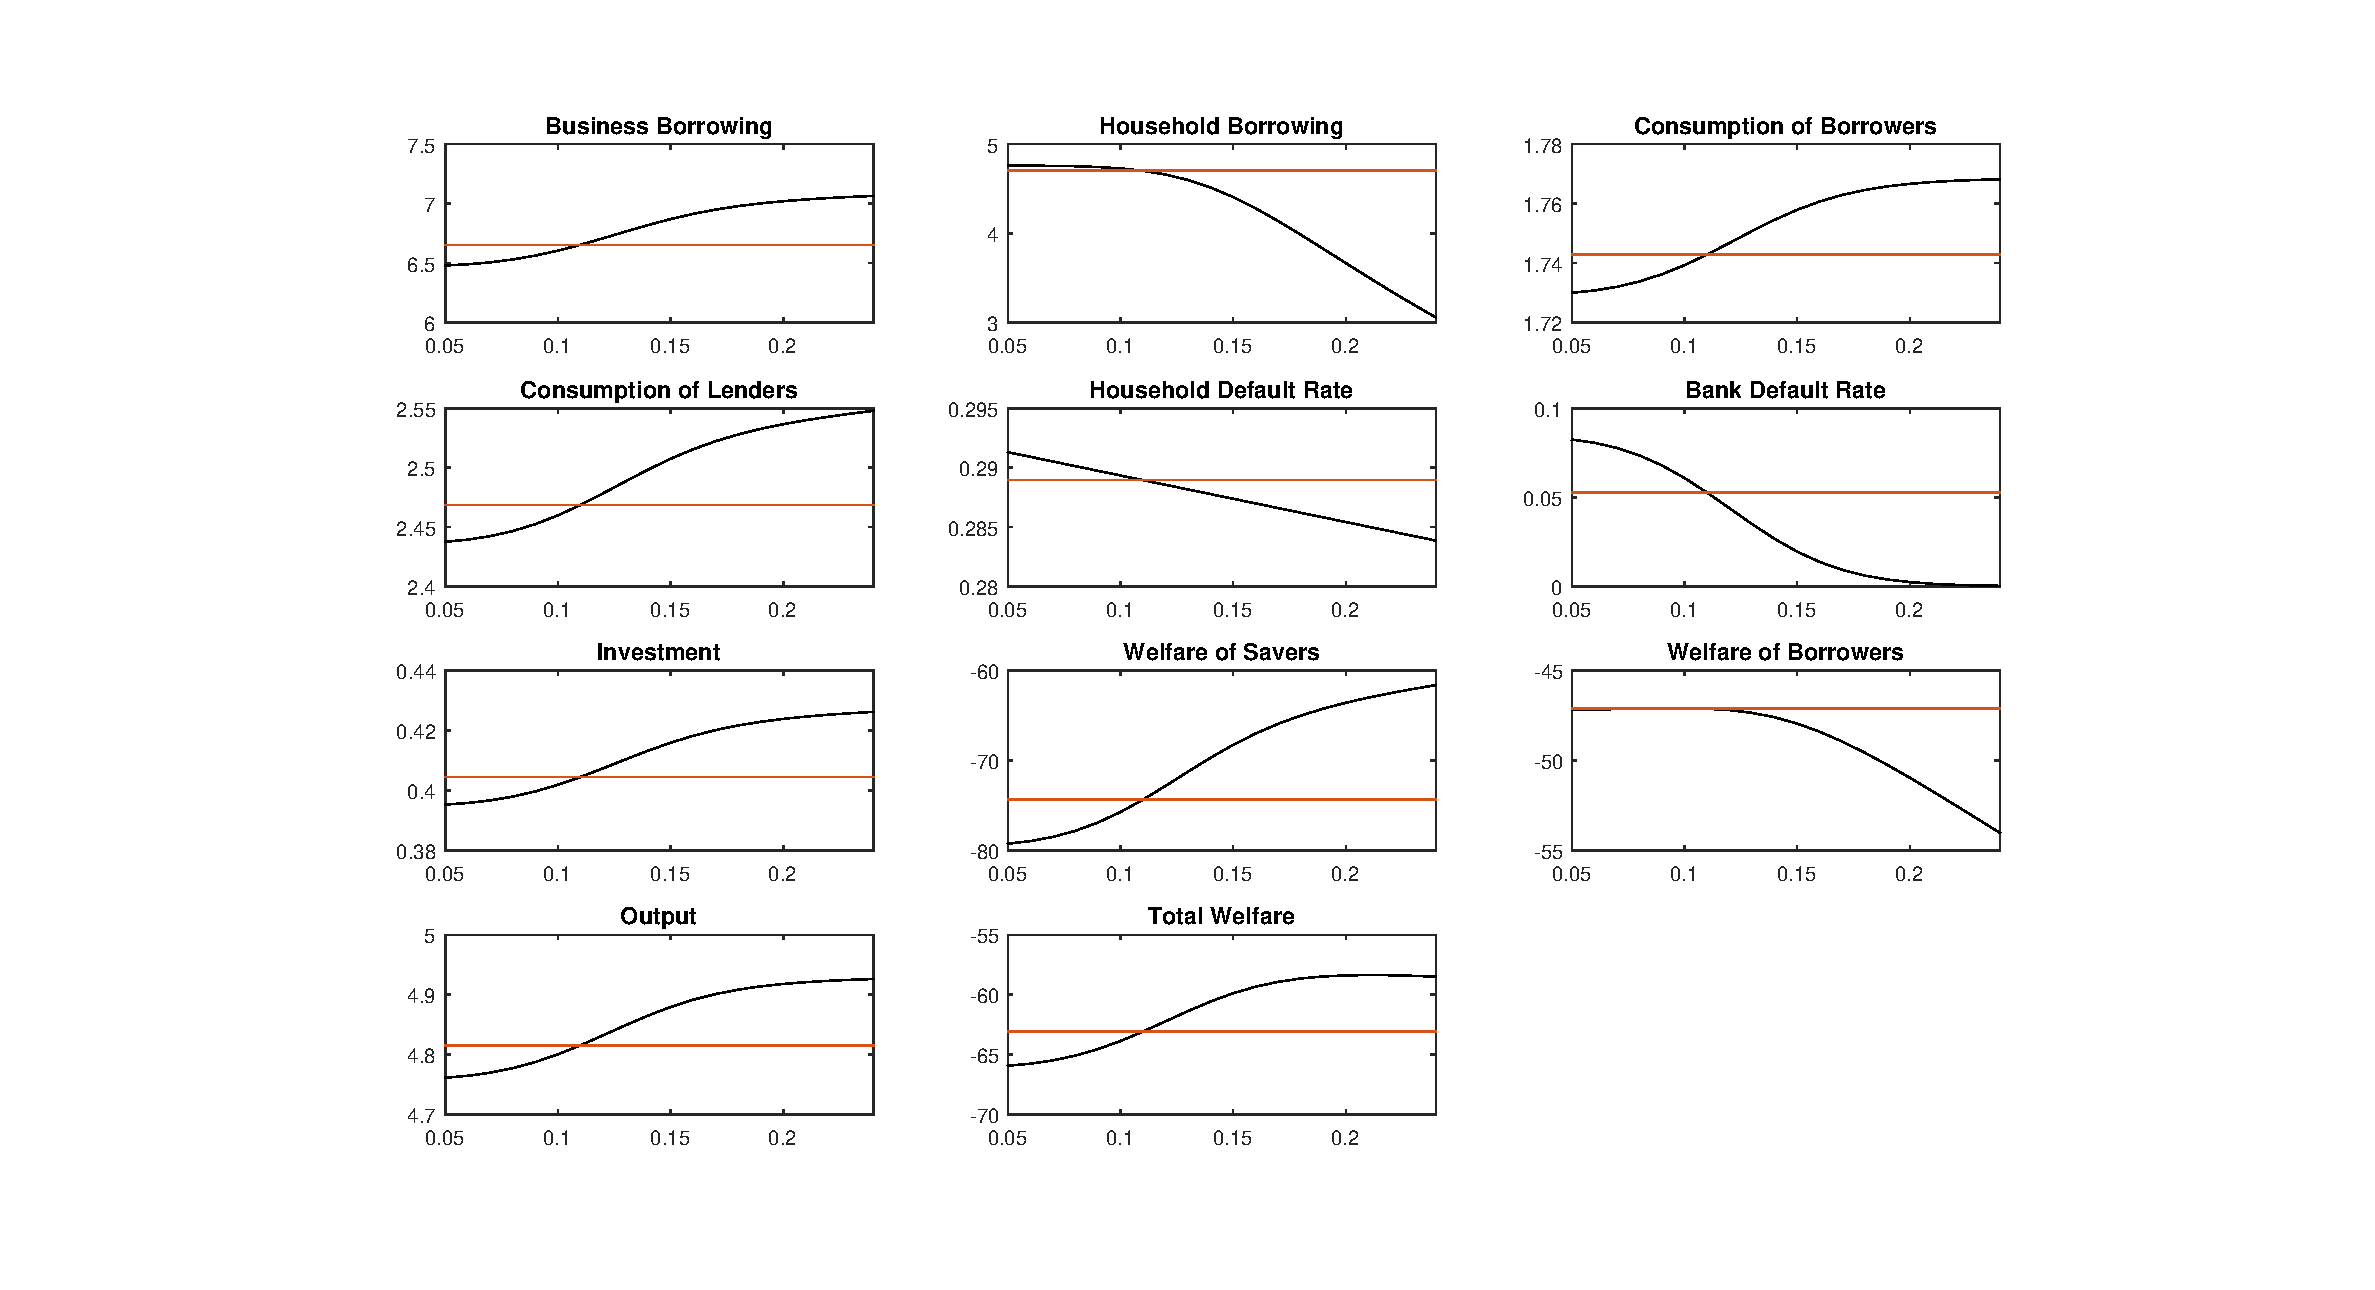
\includegraphics[scale=0.3]{WA_SCR_housing_level.pdf}\\

\end{figure}

\end{frame}


%\begin{frame}{Minimum Capital Requirements and Volatility}

%\begin{figure}[H]
%\centering
%\caption{Sectoral capital requirements on mortgage lending with a baseline of 11 \%. Welfare maximizing value is 20.7 \% with a weight of 0 on volatility. It decreases to 17.6 \% with a weight of 0.1 on the volatility.
%\textbf{Welfare improvement: 7.47 \% and 4.26 \% respectively.} } 
%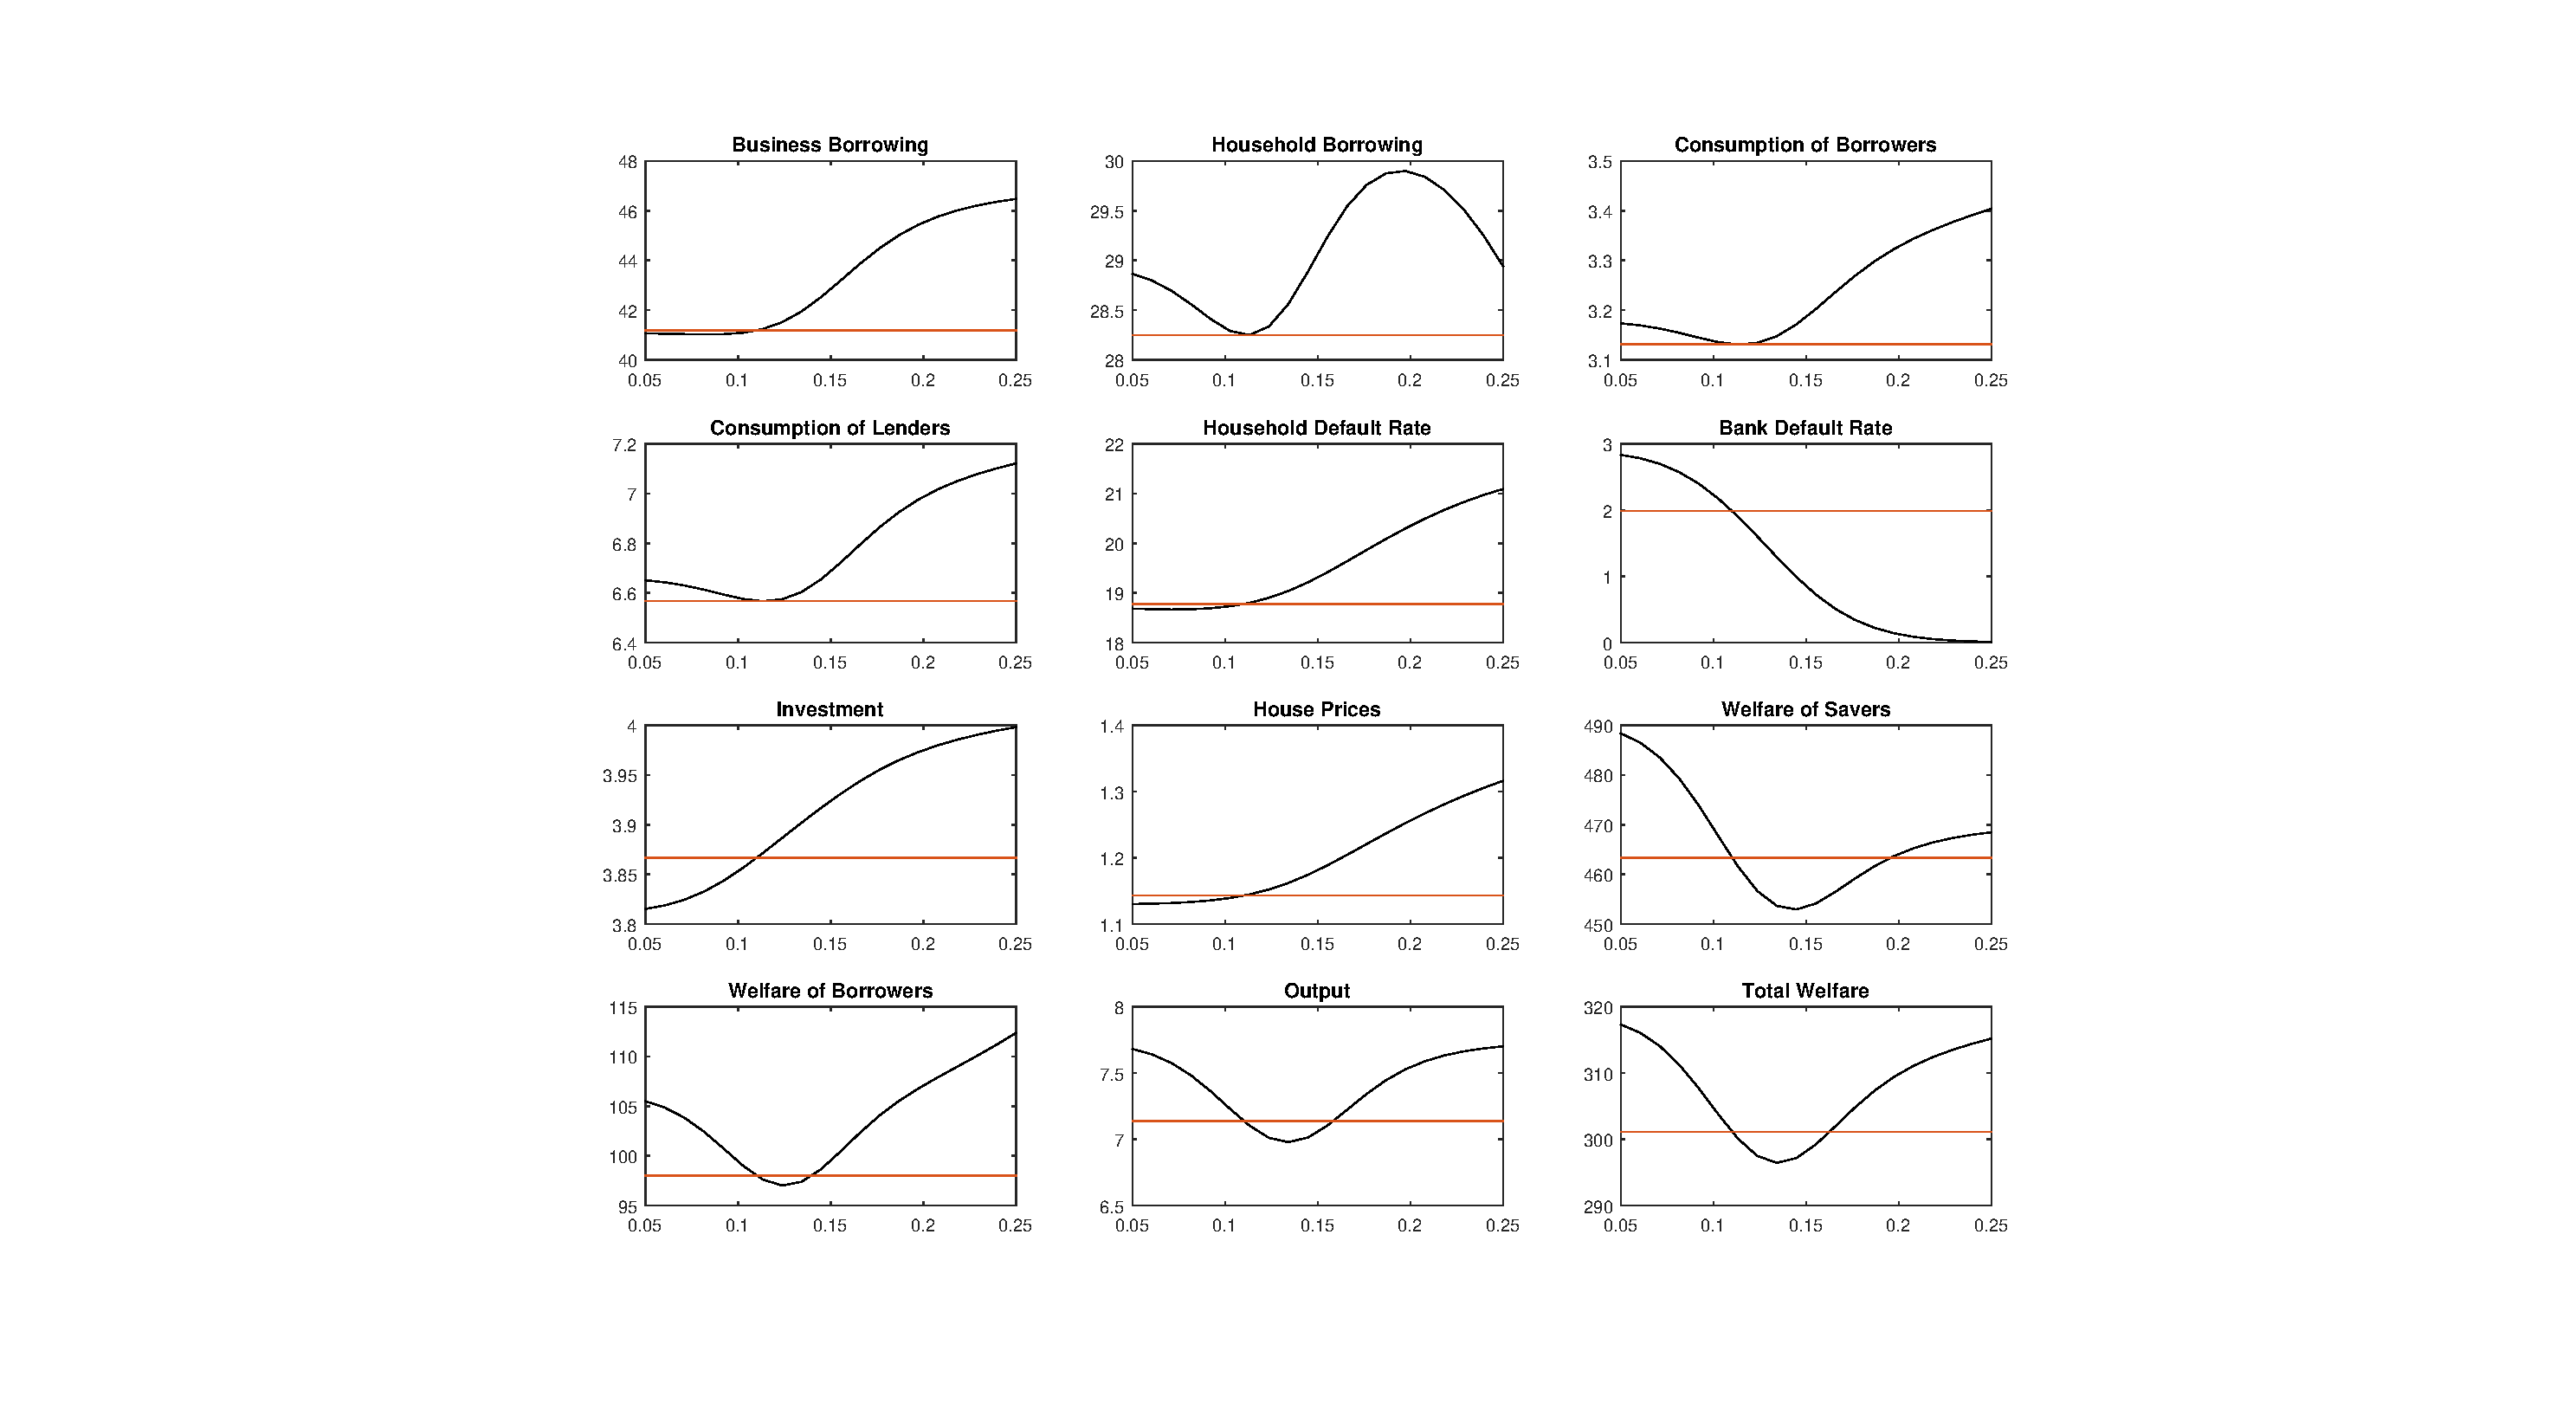
\includegraphics[scale=0.3]{WA2_var.pdf}
%\end{figure}

%\end{frame}



\begin{frame}{Optimal Policies}

\begin{itemize}
\item Ad-hoc mean-variance objective: $  E[W_t] - \omega \sqrt{Var[W_t]}  $
%\begin{itemize}
%\item Maximizing the level without introducing too much volatility.
%\end{itemize}
\end{itemize}


\pause 
\begin{table}[h]

\caption{Optimal macroprudential parameters, one at a time. Results with $\omega=0.1$. 
Benchmark values are: 11 \% for CAR, 86 \% for LTV limit, no SCR. }
\begin{tabular}{l|l|l}

 \hline
 \hline
Parameter   &  Optimal Value & Welfare Improvement \\
\hline
\hline
LTV Limit&    86.6 \%  & 0.001 \%  \\

SCR-Mortgage &    17.6 \% (11 \% CAR, 6.6 \% add-on) & 4.26 \% \\

SCR-Corporate &    16.7 \% (11 \% CAR, 5.7 \% add-on) & 3.22 \% \\

CAR &    14.5 \% & 3.82 \% \\

%CCyB &    Max. attainable \\

\end{tabular}
\end{table}

\pause

\begin{table}[h]

\caption{Optimal joint SCRs and LTV}
\begin{tabular}{l|l}

 \hline
 \hline
Parameter  &  \\
\hline
\hline
LTV &    94.06 \%  \\

SCR-Mortgage      & 15.88 \%  \\

SCR-Corporate \%  & 12.5 \%  \\

Welfare Improvement  & 4.8 \% \\

\end{tabular}
\end{table}

\begin{itemize}
%\item \textbf{SCR-Mortgage requirements play a dominant role.} 
\item \textbf{Larger improvement with lower SCRs when macroprudential tools are coordinated.} 
\item {LTV limit can be relaxed if SCRs are sufficiently high. }
\item CCyB is not as effective as CAR \& SCRs. 
\end{itemize}

\end{frame}




\begin{frame}{Counterfactual with optimized policies}
\begin{figure}[H]
\centering
\caption{Counterfactual I with optimized values: $\phi_H=15.8 \%, \phi_F=12.5 \%, \epsilon_H=94 \%$.}
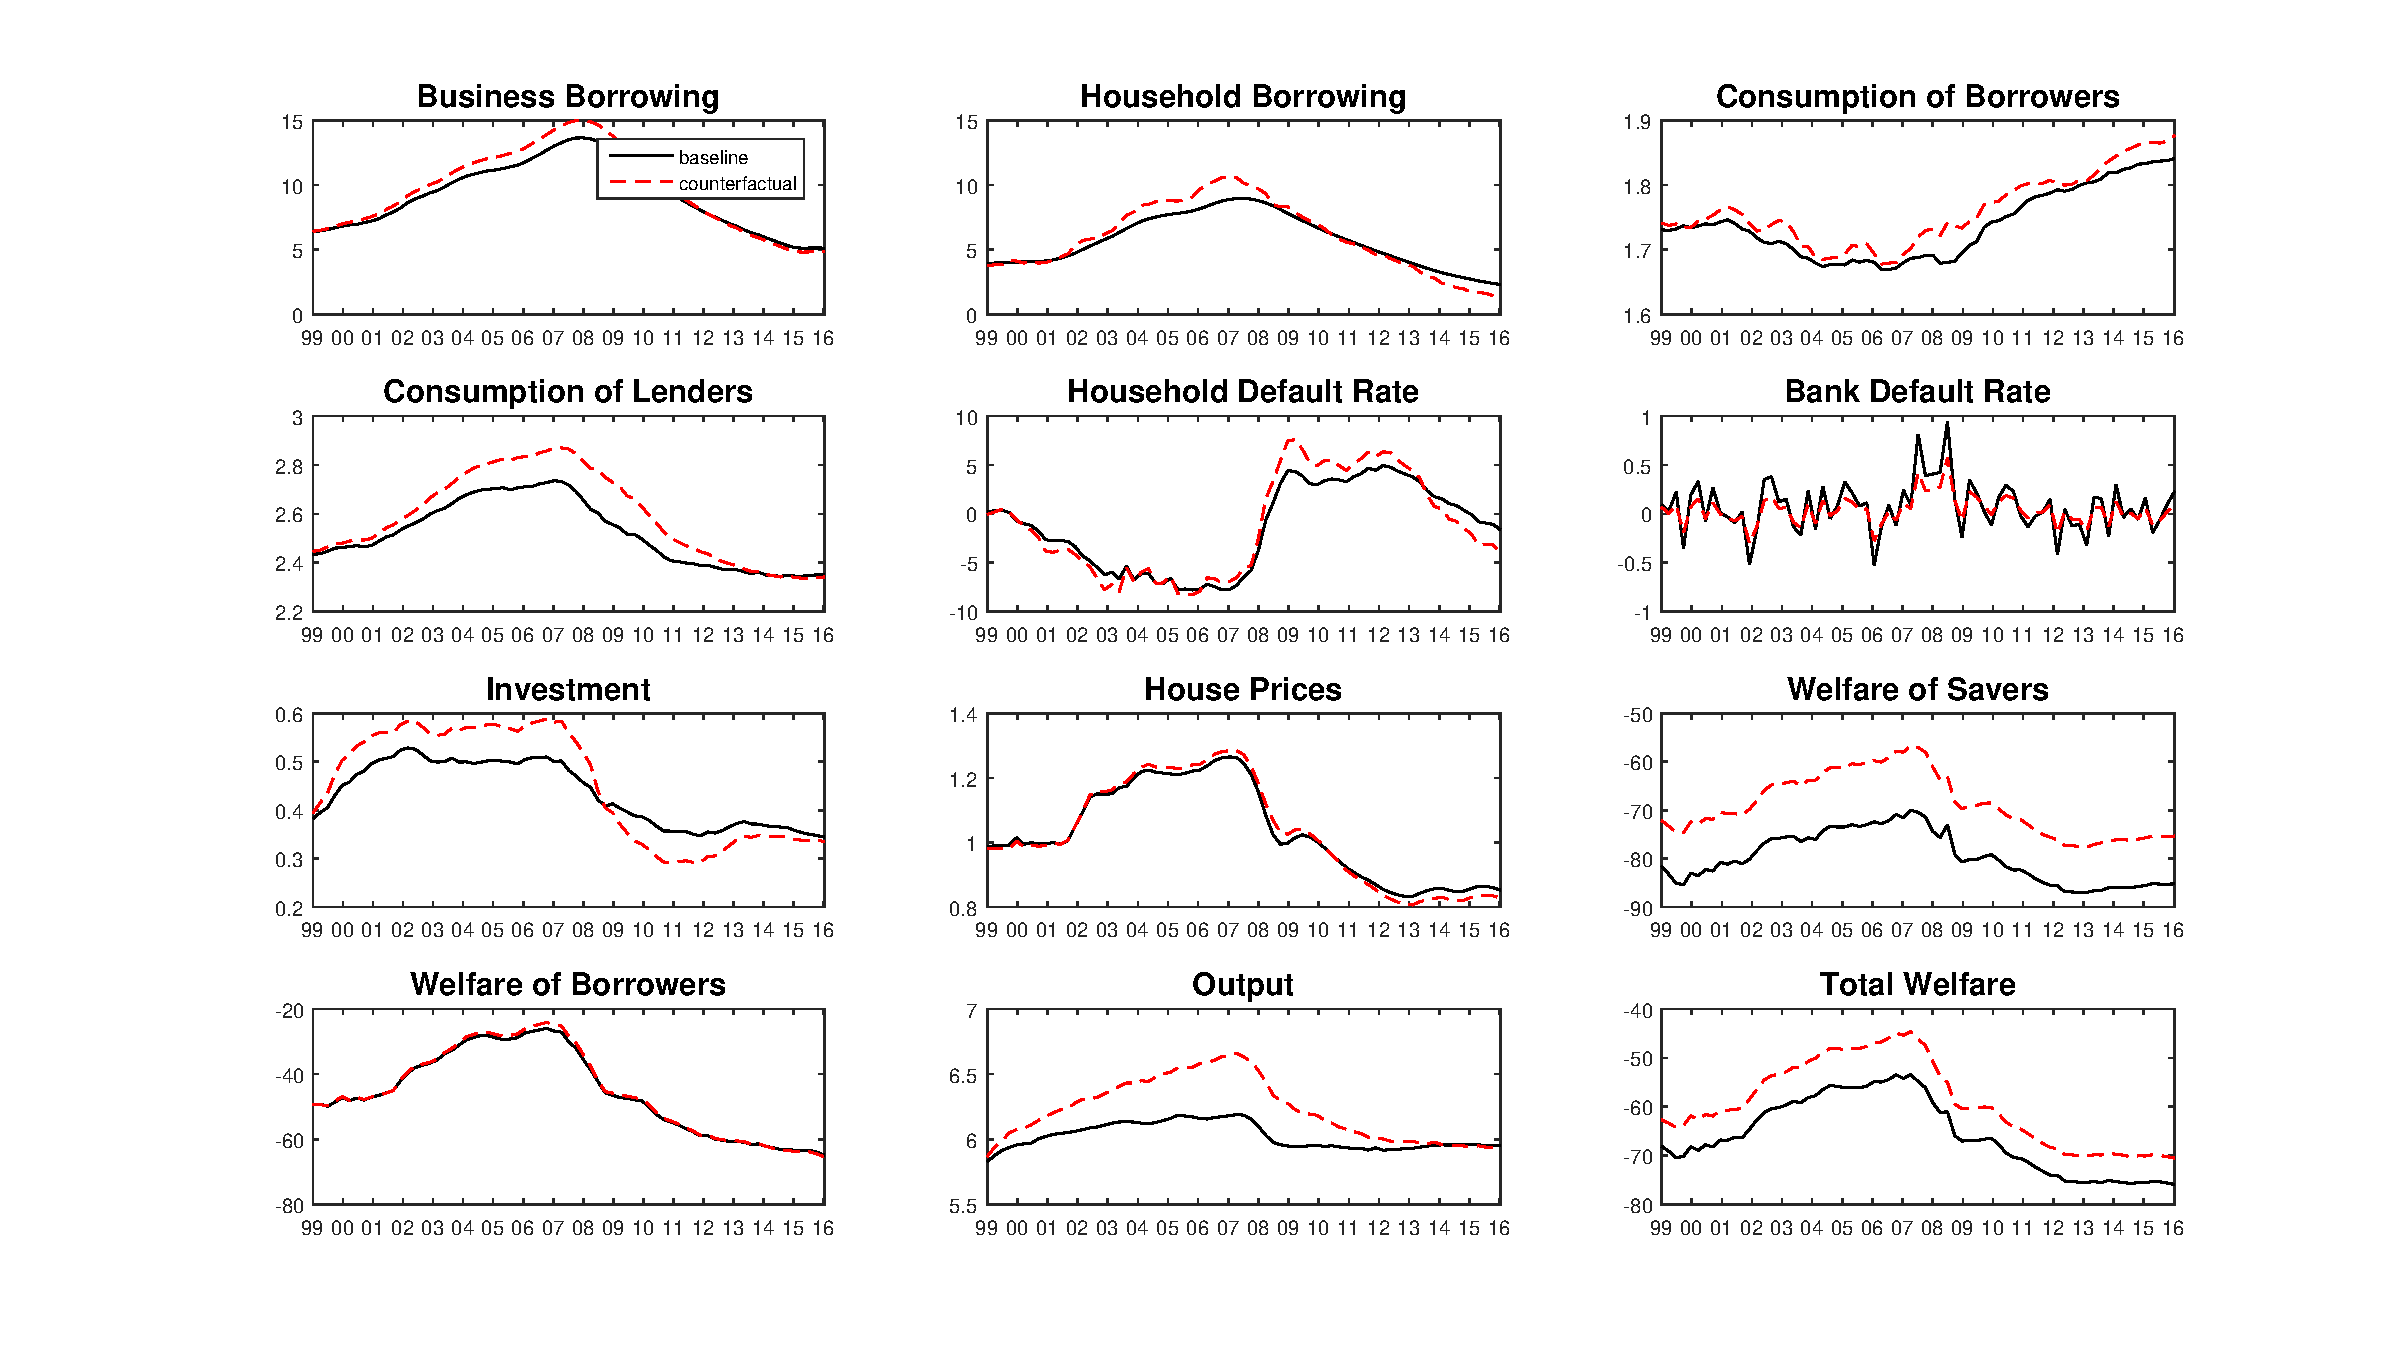
\includegraphics[scale=0.25]{counterfactuals2.pdf}
\end{figure}
\end{frame}

\begin{frame}{Counterfactual with CCyB}
\begin{figure}[H]
\centering
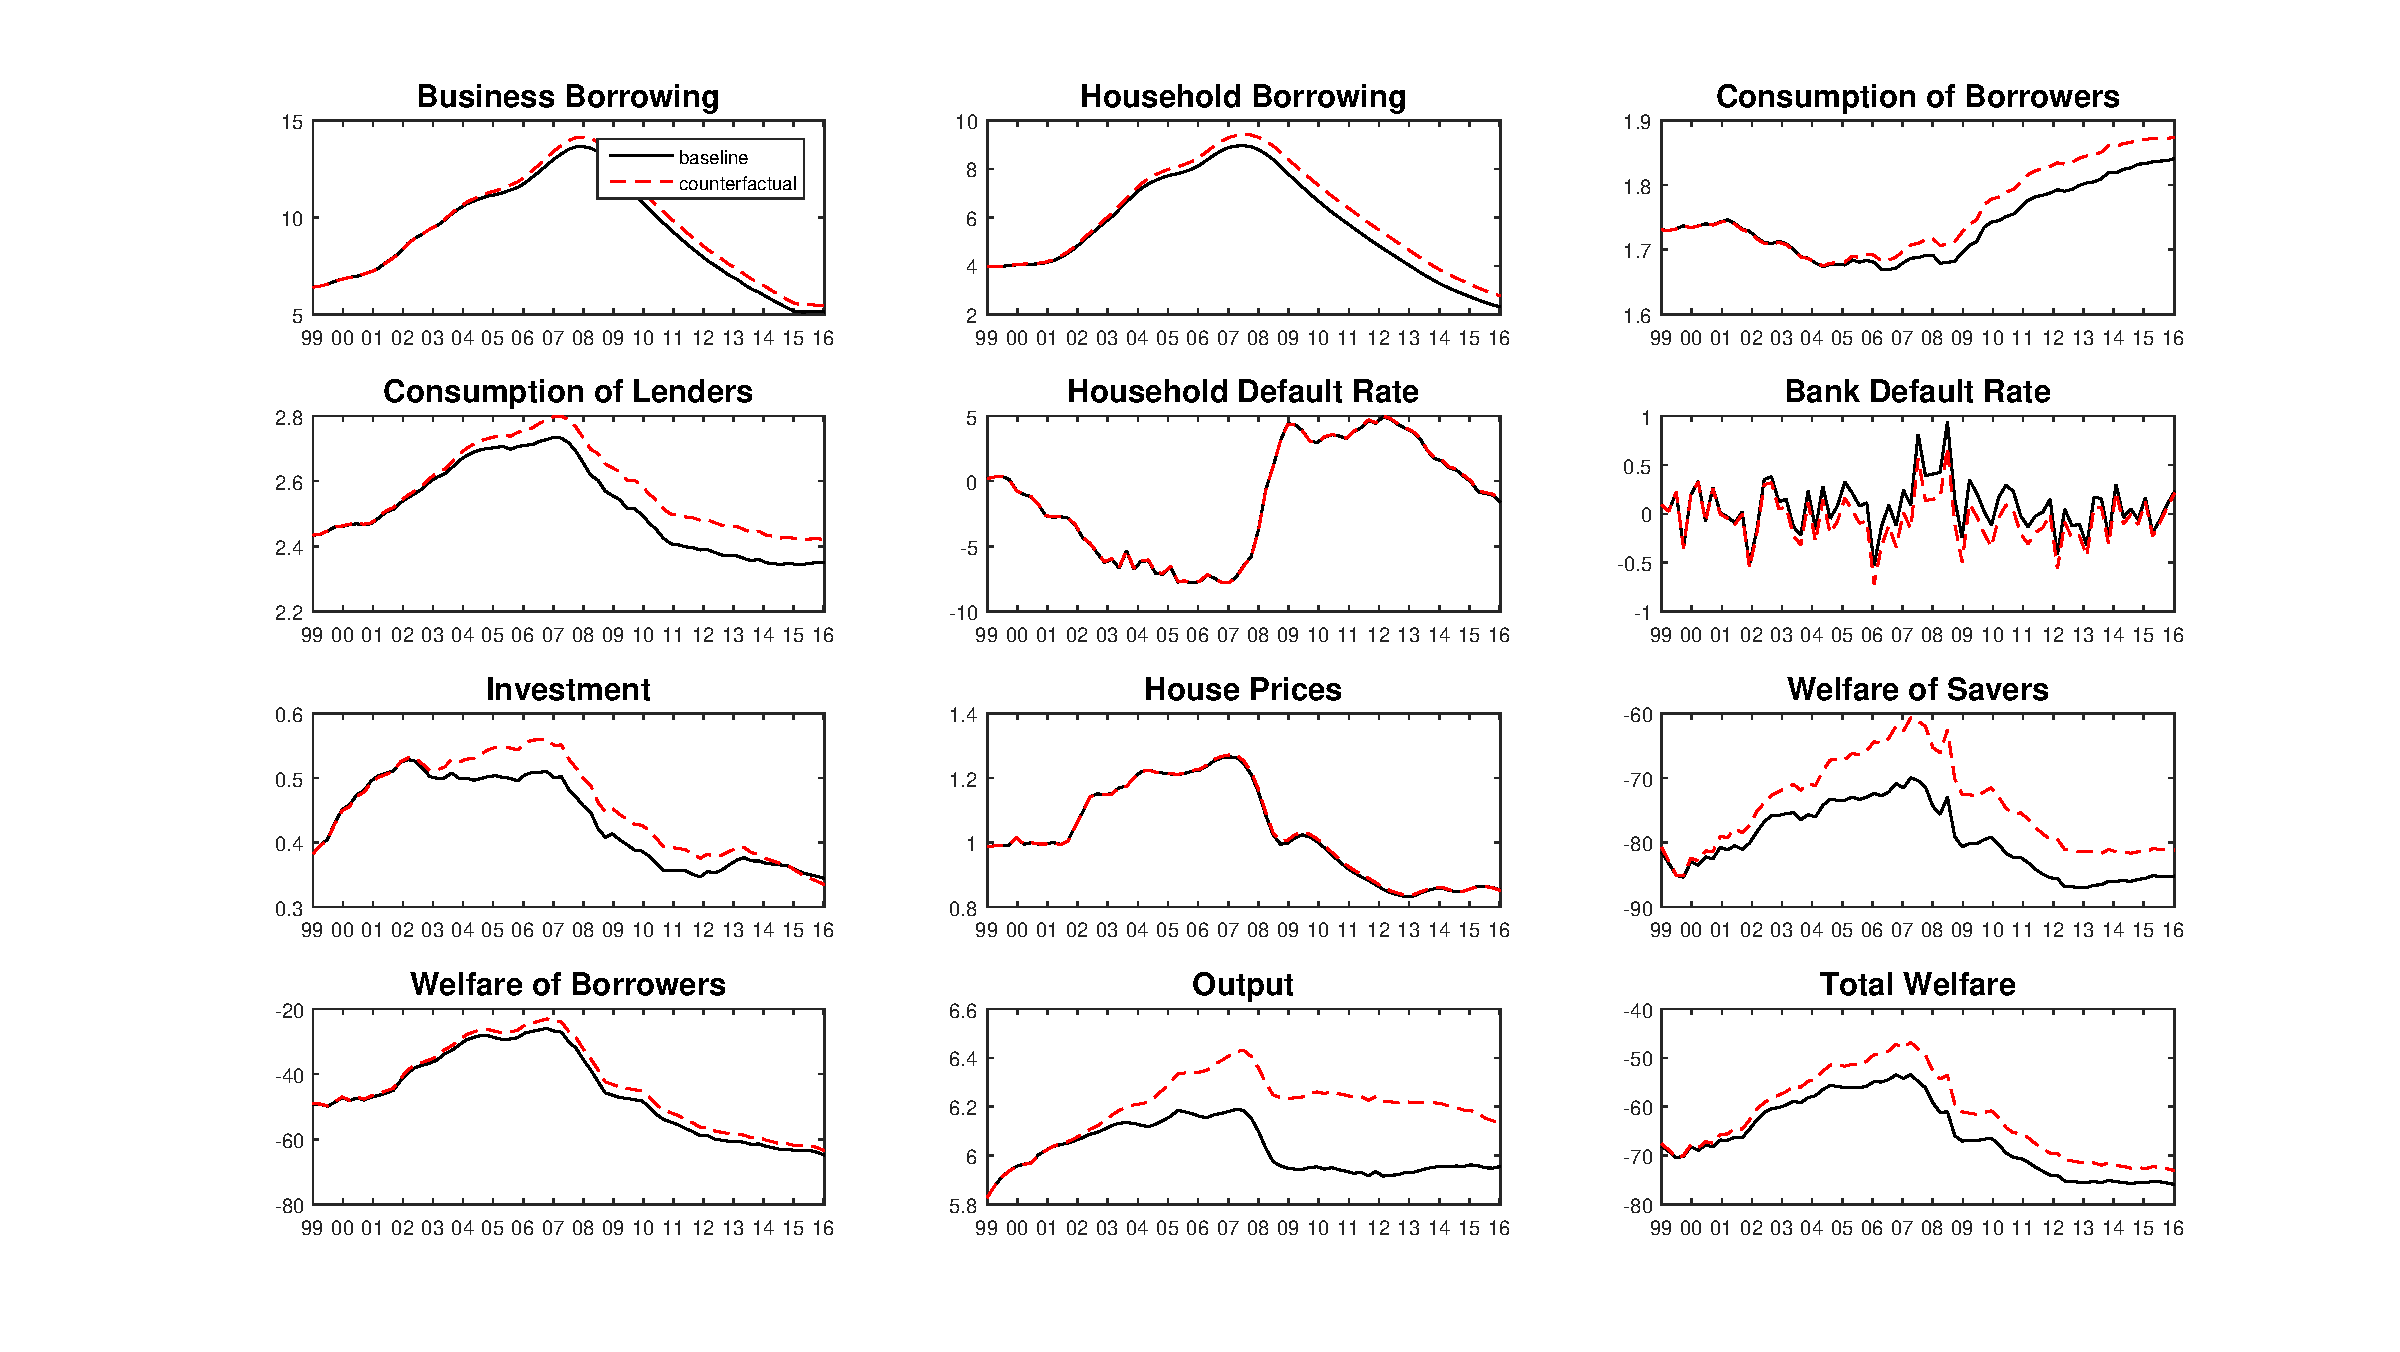
\includegraphics[scale=0.25]{counterfactualsccyb.pdf}
\end{figure}
\end{frame}




%\begin{frame}{Counterfactual II: Phasing-in}
%\begin{figure}[H]
%\centering
%\caption{Same counterfactual phased-in over a 5-year period over 2001-2006 in equal increments.}
%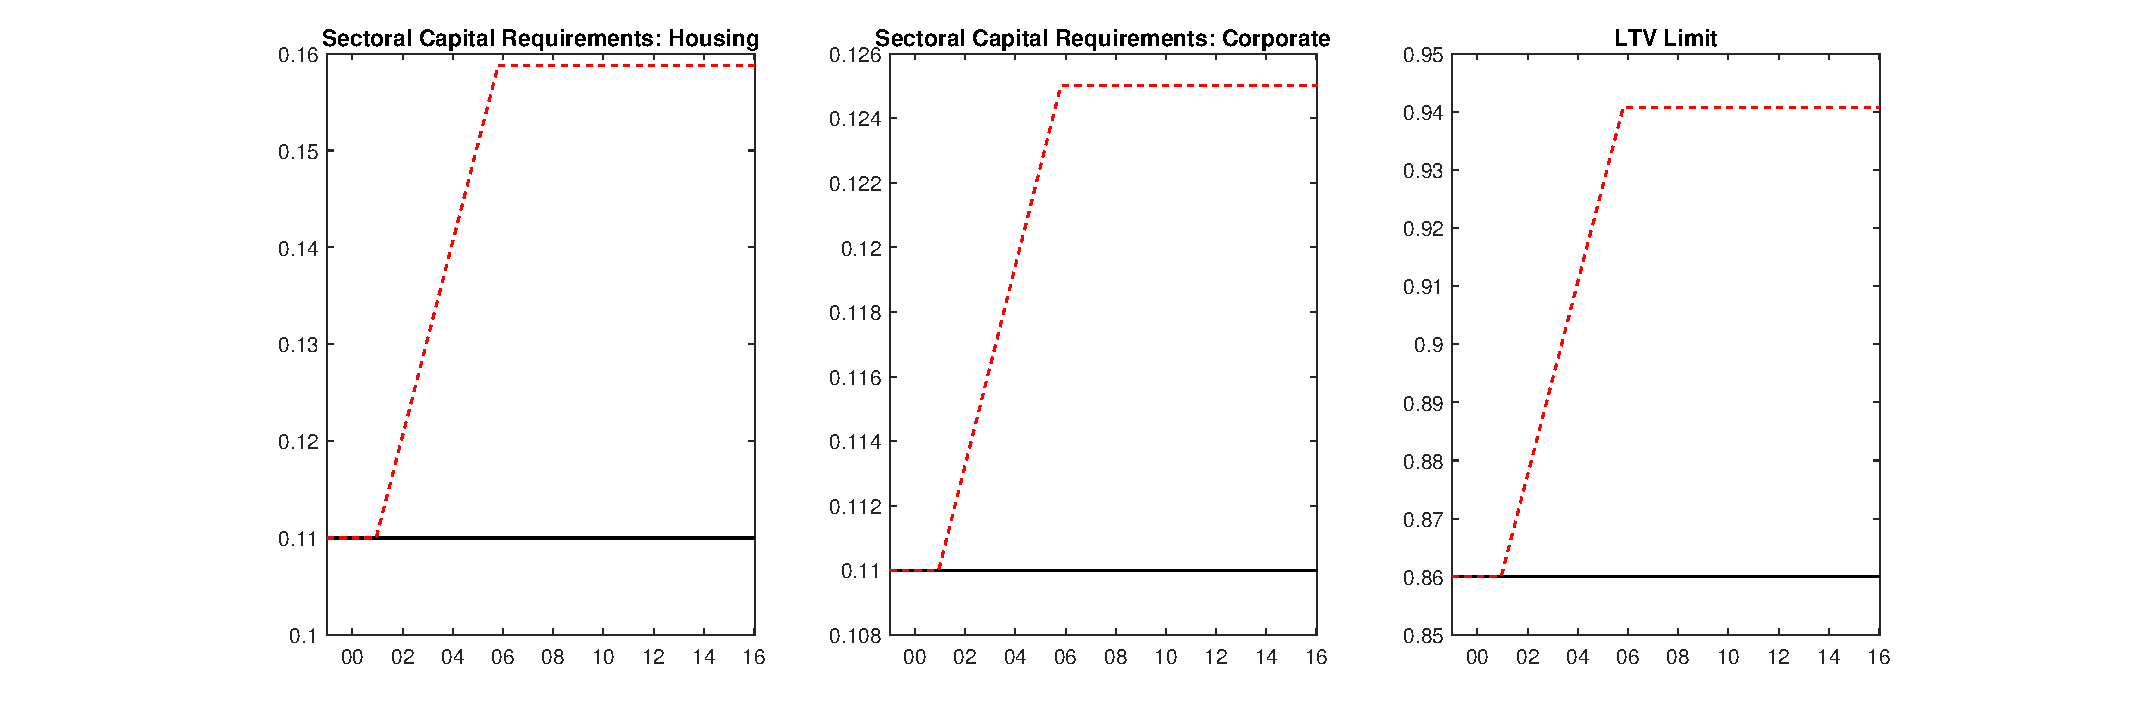
\includegraphics[scale=0.35]{CF_policy_rules10.pdf}
%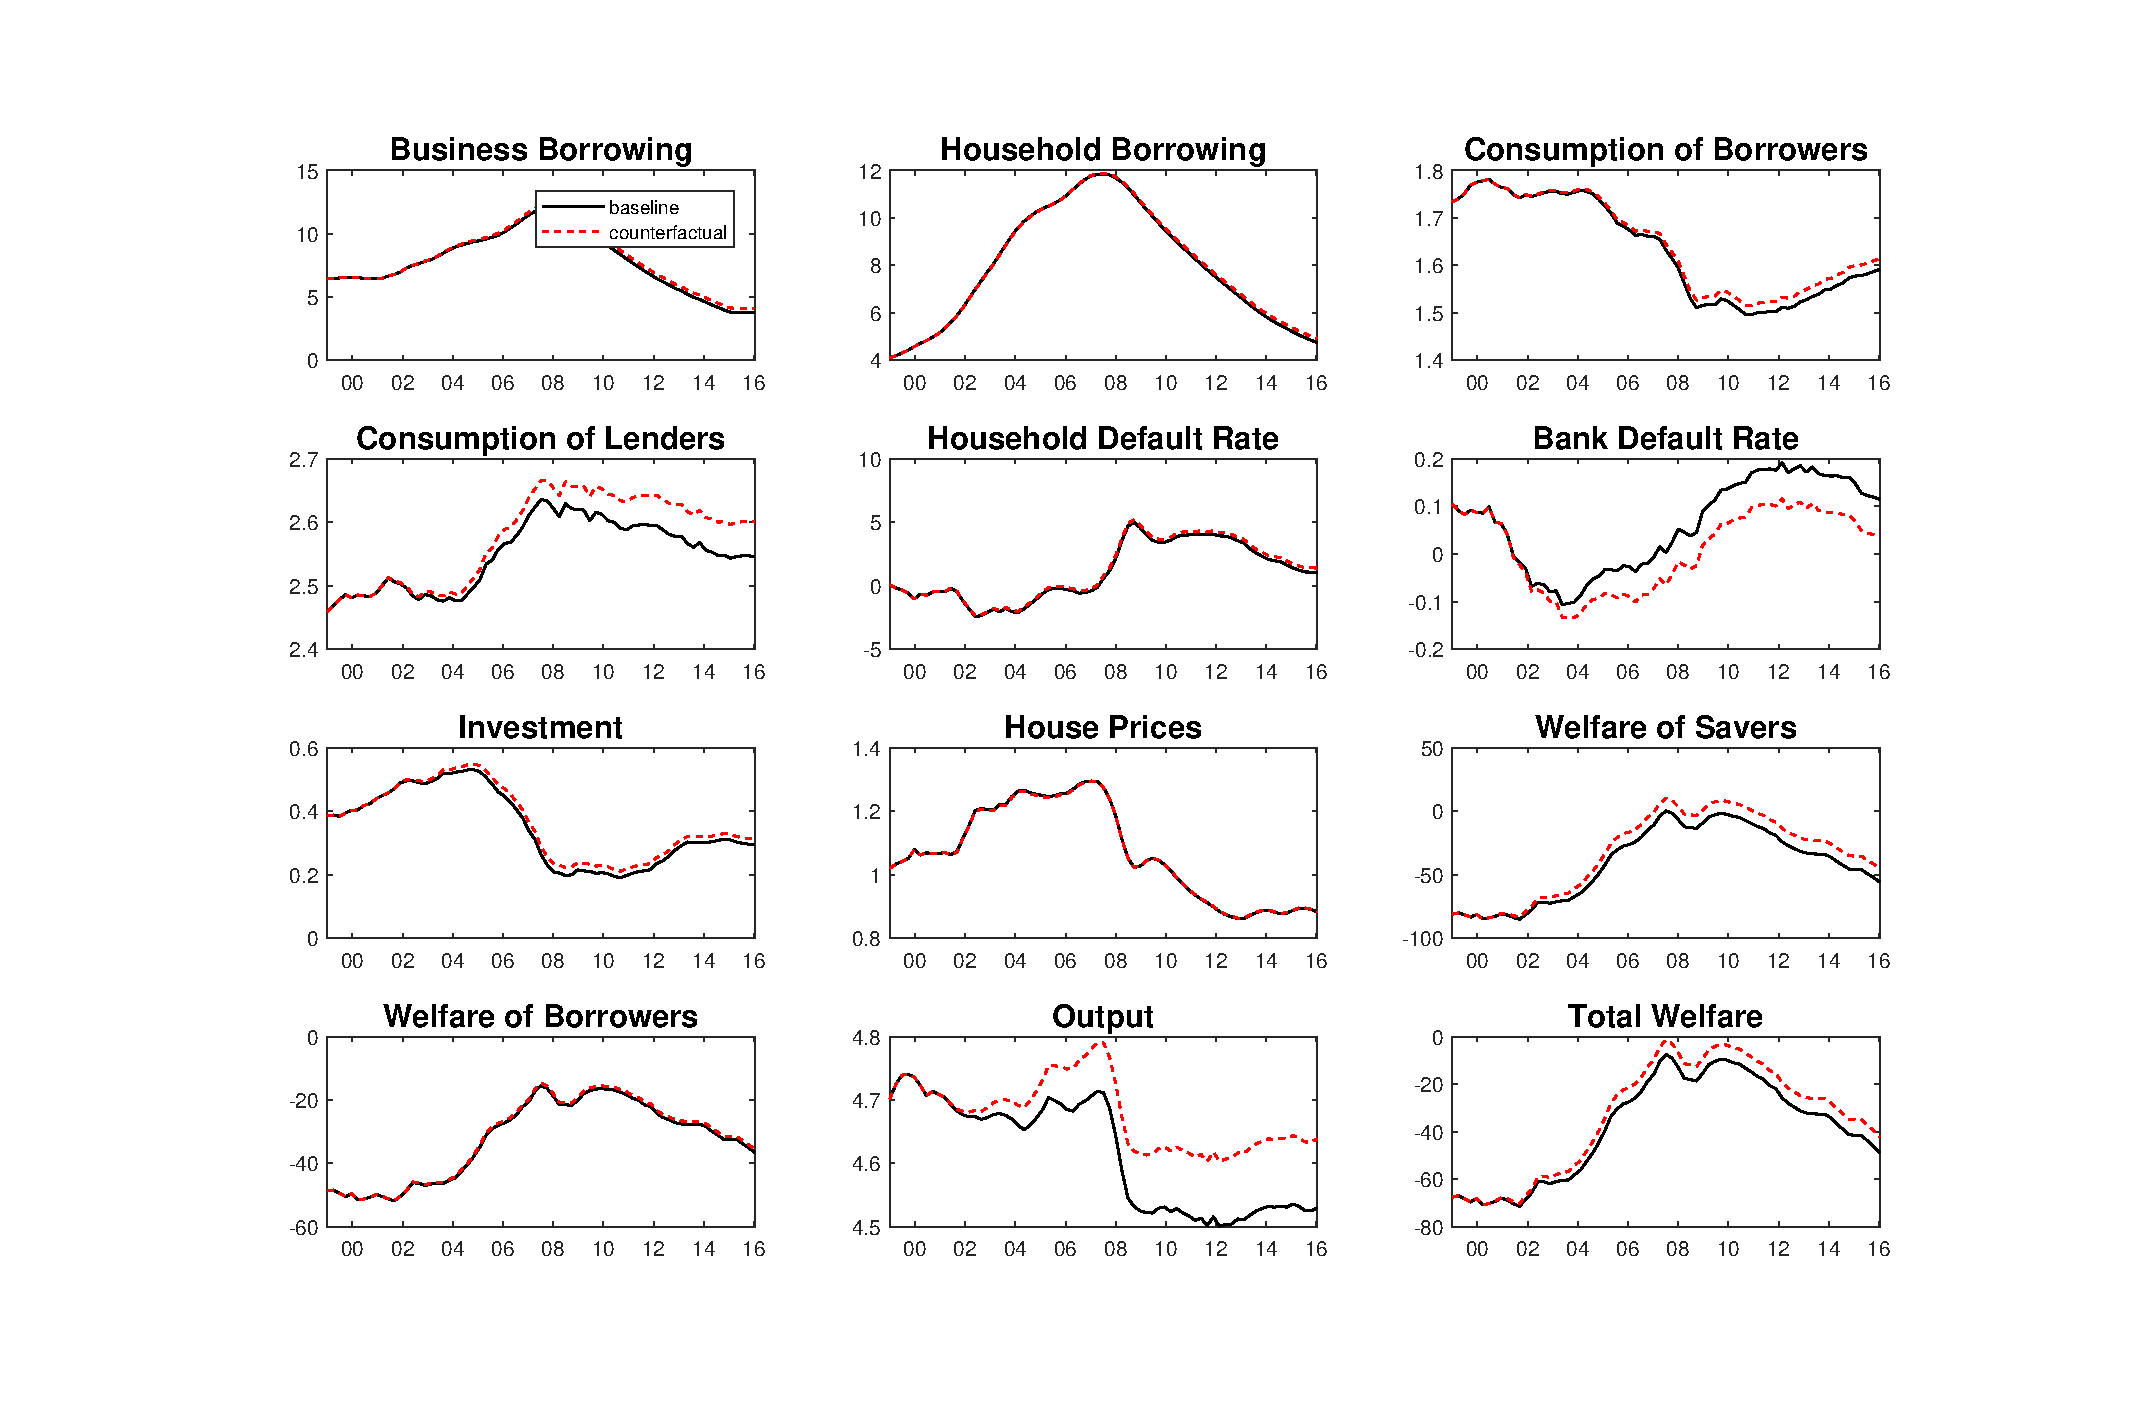
\includegraphics[scale=0.45]{counterfactuals10.pdf}\\
%\end{figure}
%\end{frame}


%\begin{frame}{Changes in the Level and Volatility}

%\begin{table}[h]
%\caption{Policies introduced at once at the beginning of the sample. }
%\begin{tabular}{l|l|l}
%Variable &  Change in Level &  Change in Volatility \\
%\hline
%\hline
%    Corporate Credit           &       0.039    &      0.041 \\
%    Mortgage Credit            &      0.024    &       0.147 \\
%    Output         &     0.019    &    -0.0354 \\ 
%    Household Welfare       &     0.175     &     0.0437\\
%\end{tabular}
%\end{table}

%\pause 

%\begin{table}[h]
%\caption{Policies phased-in over 2001-2006.}
%\begin{tabular}{l|l|l}
%\small
%Variable &  Change in Level &  Change in Volatility \\
%\hline
%\hline
%    Corporate Credit           &       0.024    &      -0.001 \\
%    Mortgage Credit            &      0.006    &       -0.007 \\
%    Output                      &     0.014    &    -0.0356 \\ 
%    Household Welfare       &     0.12     &     0.096\\
%\end{tabular}
%\end{table}

%\pause 


%\begin{table}[h]
%\caption{Policies phased-in over 2001-2006, without interest rate stickiness.}
%\begin{tabular}{l|l|l}
%\small
%Variable &  Change in Level & Change in Volatility \\
%\hline
%\hline
%    Corporate Credit           &       0.041    &     0.02 \\
%    Mortgage Credit            &      0.029    &      0.08 \\
%    Output                      &     0.02    &    -0.028 \\ 
%    Household Welfare       &     0.12     &     0.098\\
%\end{tabular}
%\end{table}
%\end{frame}

%\begin{frame}{Interface}
%\begin{itemize}
%\item Most policy experiments are available in our user interface. 
%\end{itemize}
%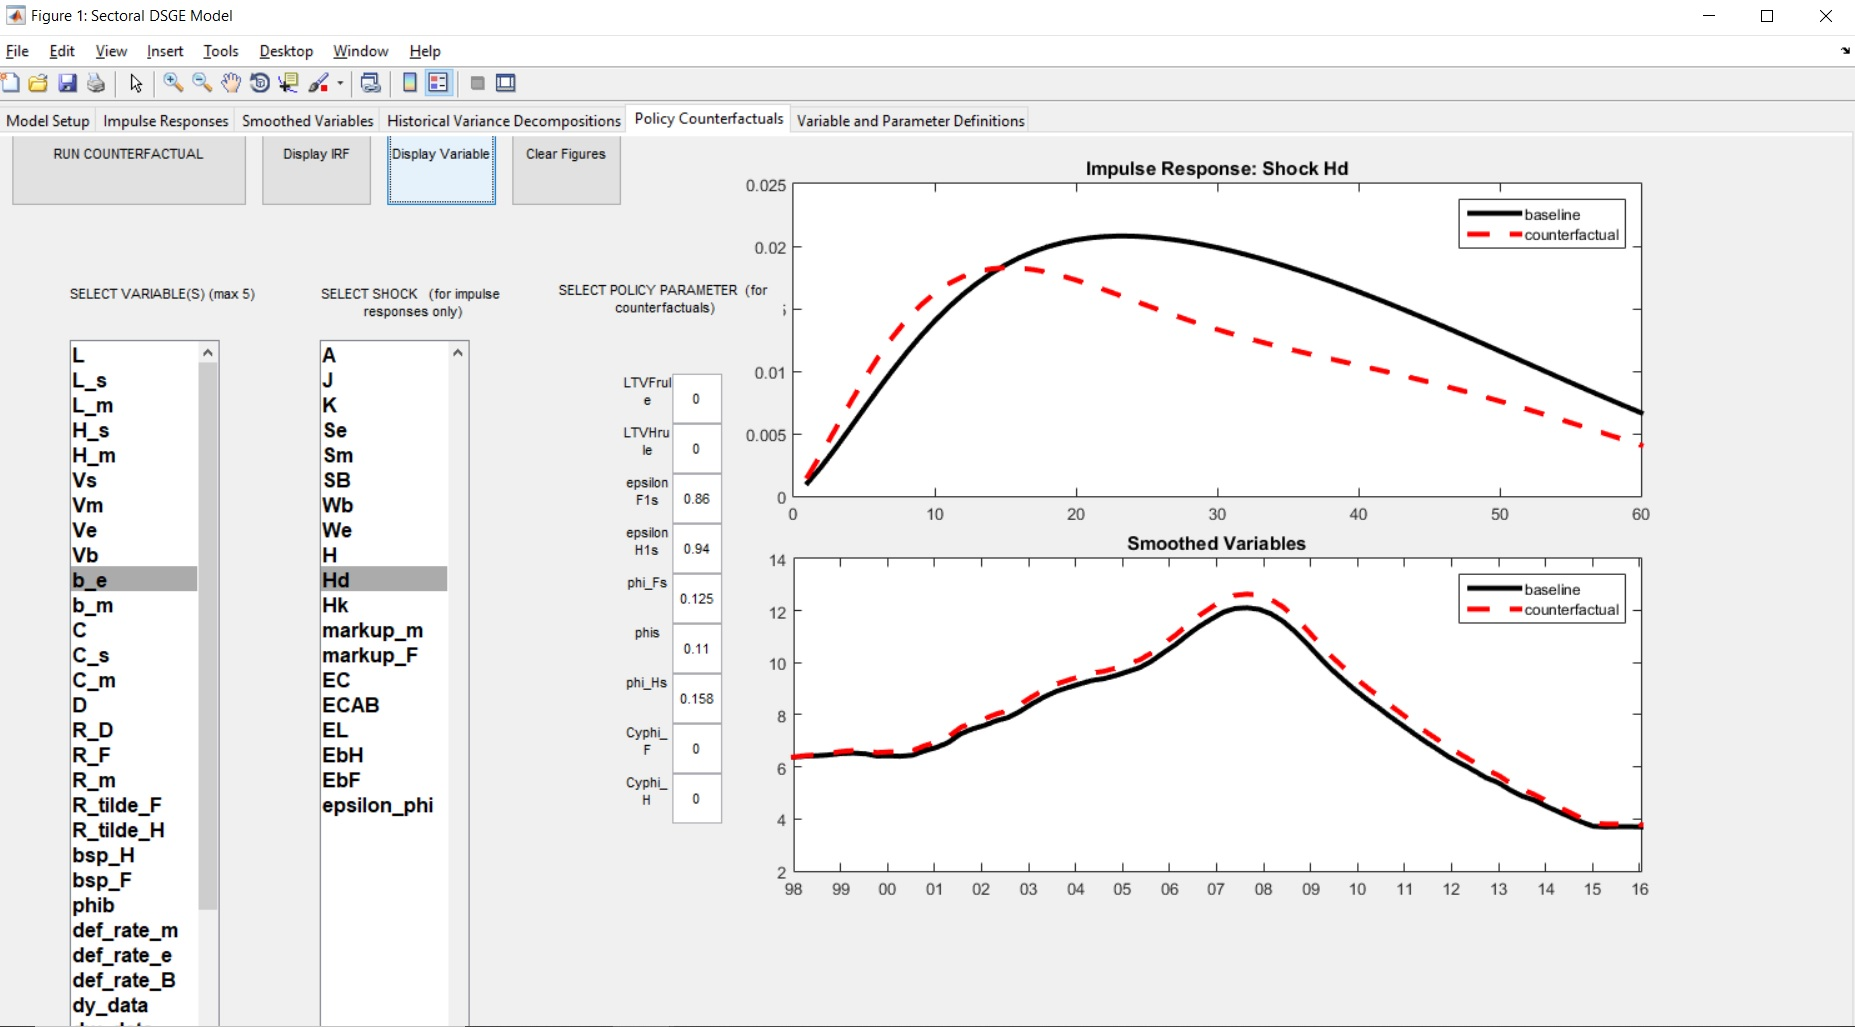
\includegraphics[scale=0.3]{gui_screenshot.jpg}
%\end{frame}












%\begin{frame}{Interest Rate Pass-through \& Prudential Policy Interactions}

%\begin{itemize}
%\item The impact of macroprudential tools will be weaker in cases where interest rate stickiness is high. 
%\end{itemize}

%\begin{figure}[H]
%\caption{Positive housing depreciation shock.  }
%Cumulative differences: 0.14 \% and 0.59 \%.
%\subfigure[Impact of CCyB with and without interest-rate stickiness]{\includegraphics[scale=0.15]{stickiness_ccybHd.pdf}}
%\subfigure[Impact of LTV limit with and without interest-rate stickiness]{\includegraphics[scale=0.15]{stickiness_LTVHd.pdf}}
%Cumulative differences: 3.23 \% and 0.38 \%.
%\subfigure[Impact of CAR with and without interest-rate stickiness]{\includegraphics[scale=0.15]{stickiness_CARHd.pdf}}
%\end{figure}
%\end{frame}


%\begin{frame}{Conclusions \& Future Work}


%\begin{itemize}
%\item Conclusions:
%\vspace{3 mm}
%\begin{itemize}
%\item Coordination of macroprudential tools may have a welfare improving effect
%\vspace{3 mm}
%\item macroprudential tools would have improved some macroeconomic indicators but not have prevented the crisis altogether
%\vspace{3 mm}
%\item Interest rate sluggishness may weaken the transmission of macroprudential tools that work through interest rates
%\end{itemize}

\begin{comment}

\vspace{5 mm}
\item Future work: 
\vspace{3 mm}
\begin{itemize}
\item Interaction between LTI \& LTV limits
\vspace{3 mm}
\item Introduction of monetary policy 
\vspace{3 mm}
\item Household heterogeneity 

\begin{itemize}
\item The impact of heterogeneous expectations on the effectiveness of macroprudential tools
\end{itemize}
\end{itemize}

\end{itemize}
\end{frame}

\begin{frame}{Appendix-Estimation Details}

\begin{itemize}
\item \textbf{State-space system:} \\
\vspace{5 mm}
$
\begin{cases}
 \textit{Model}: X_t = f(E_tX_{t+1},X_{t-1},\epsilon_t)   \\
 \textit{Measurement equations}: y_t = F X_t
\end{cases}
$
\vspace{5 mm}
\item Estimation steps: 


\begin{itemize}
\item Log-linearize around the steady-state 
\vspace{5 mm}
\item Kalman filter for the log-linearized model
\vspace{5 mm}
\item Bayesian likelihood estimation

\end{itemize}

\end{itemize}

\end{frame}


\begin{frame}{Appendix-Introducing CCyB}

\begin{itemize}
\item CCyB does not improve the outcome nearly as much as the SCRs.

\end{itemize}


\begin{table}[h]
%\caption{Does CCyB improve things when optimal SCRs are in place?}
\begin{tabular}{l|l|l}
\small
Variable & \% Change in Level & \% Change in Volatility \\
\hline
Optimal SCR+LTV & & \\
\hline
    Corporate Credit           &       0.039    &      0.041 \\
    Mortgage Credit            &      0.024    &       0.147 \\
    Output         &     0.019    &    -0.354 \\ 
    Household Welfare       &     0.175     &     0.0437\\
\end{tabular}
\end{table}



\begin{table}[h]
%\caption{Does CcyB improve things when SCRs are at their baseline value? }
\begin{tabular}{l|l|l}
\small
Variable & \% Change in Level & \% Change in Volatility \\
\hline
CCyB+Baseline SCR+LTV & & \\
\hline
    Corporate Credit           &       0.007    &      0.042 \\
    Mortgage Credit            &      0.003    &       0.029 \\
    Output         &     0.0019    &    0.37 \\ 
    Household Welfare       &     0.003     &     -0.002\\
  
 %\hline
%No Interest Stickiness & & \\
%\hline

%    Corporate Credit           &       0.016    &      0.072 \\
%    Mortgage Credit            &      0.008    &       0.108 \\
%    Output         &     0.005    &    0.675 \\ 
%    Household Welfare       &     0.013     &     -0.009\\
  \end{tabular}
\end{table}


\end{frame}




\begin{frame}{Appendix-The effect of Interest rate Stickiness on Shock Transmission-I}

\begin{itemize}
\item A shock originating in the household sector:\\
transmission to corporate side and the real economy will depend on the degree of stickiness
\end{itemize}    

\begin{figure}[H]
\centering
\caption{Negative housing preference shock}
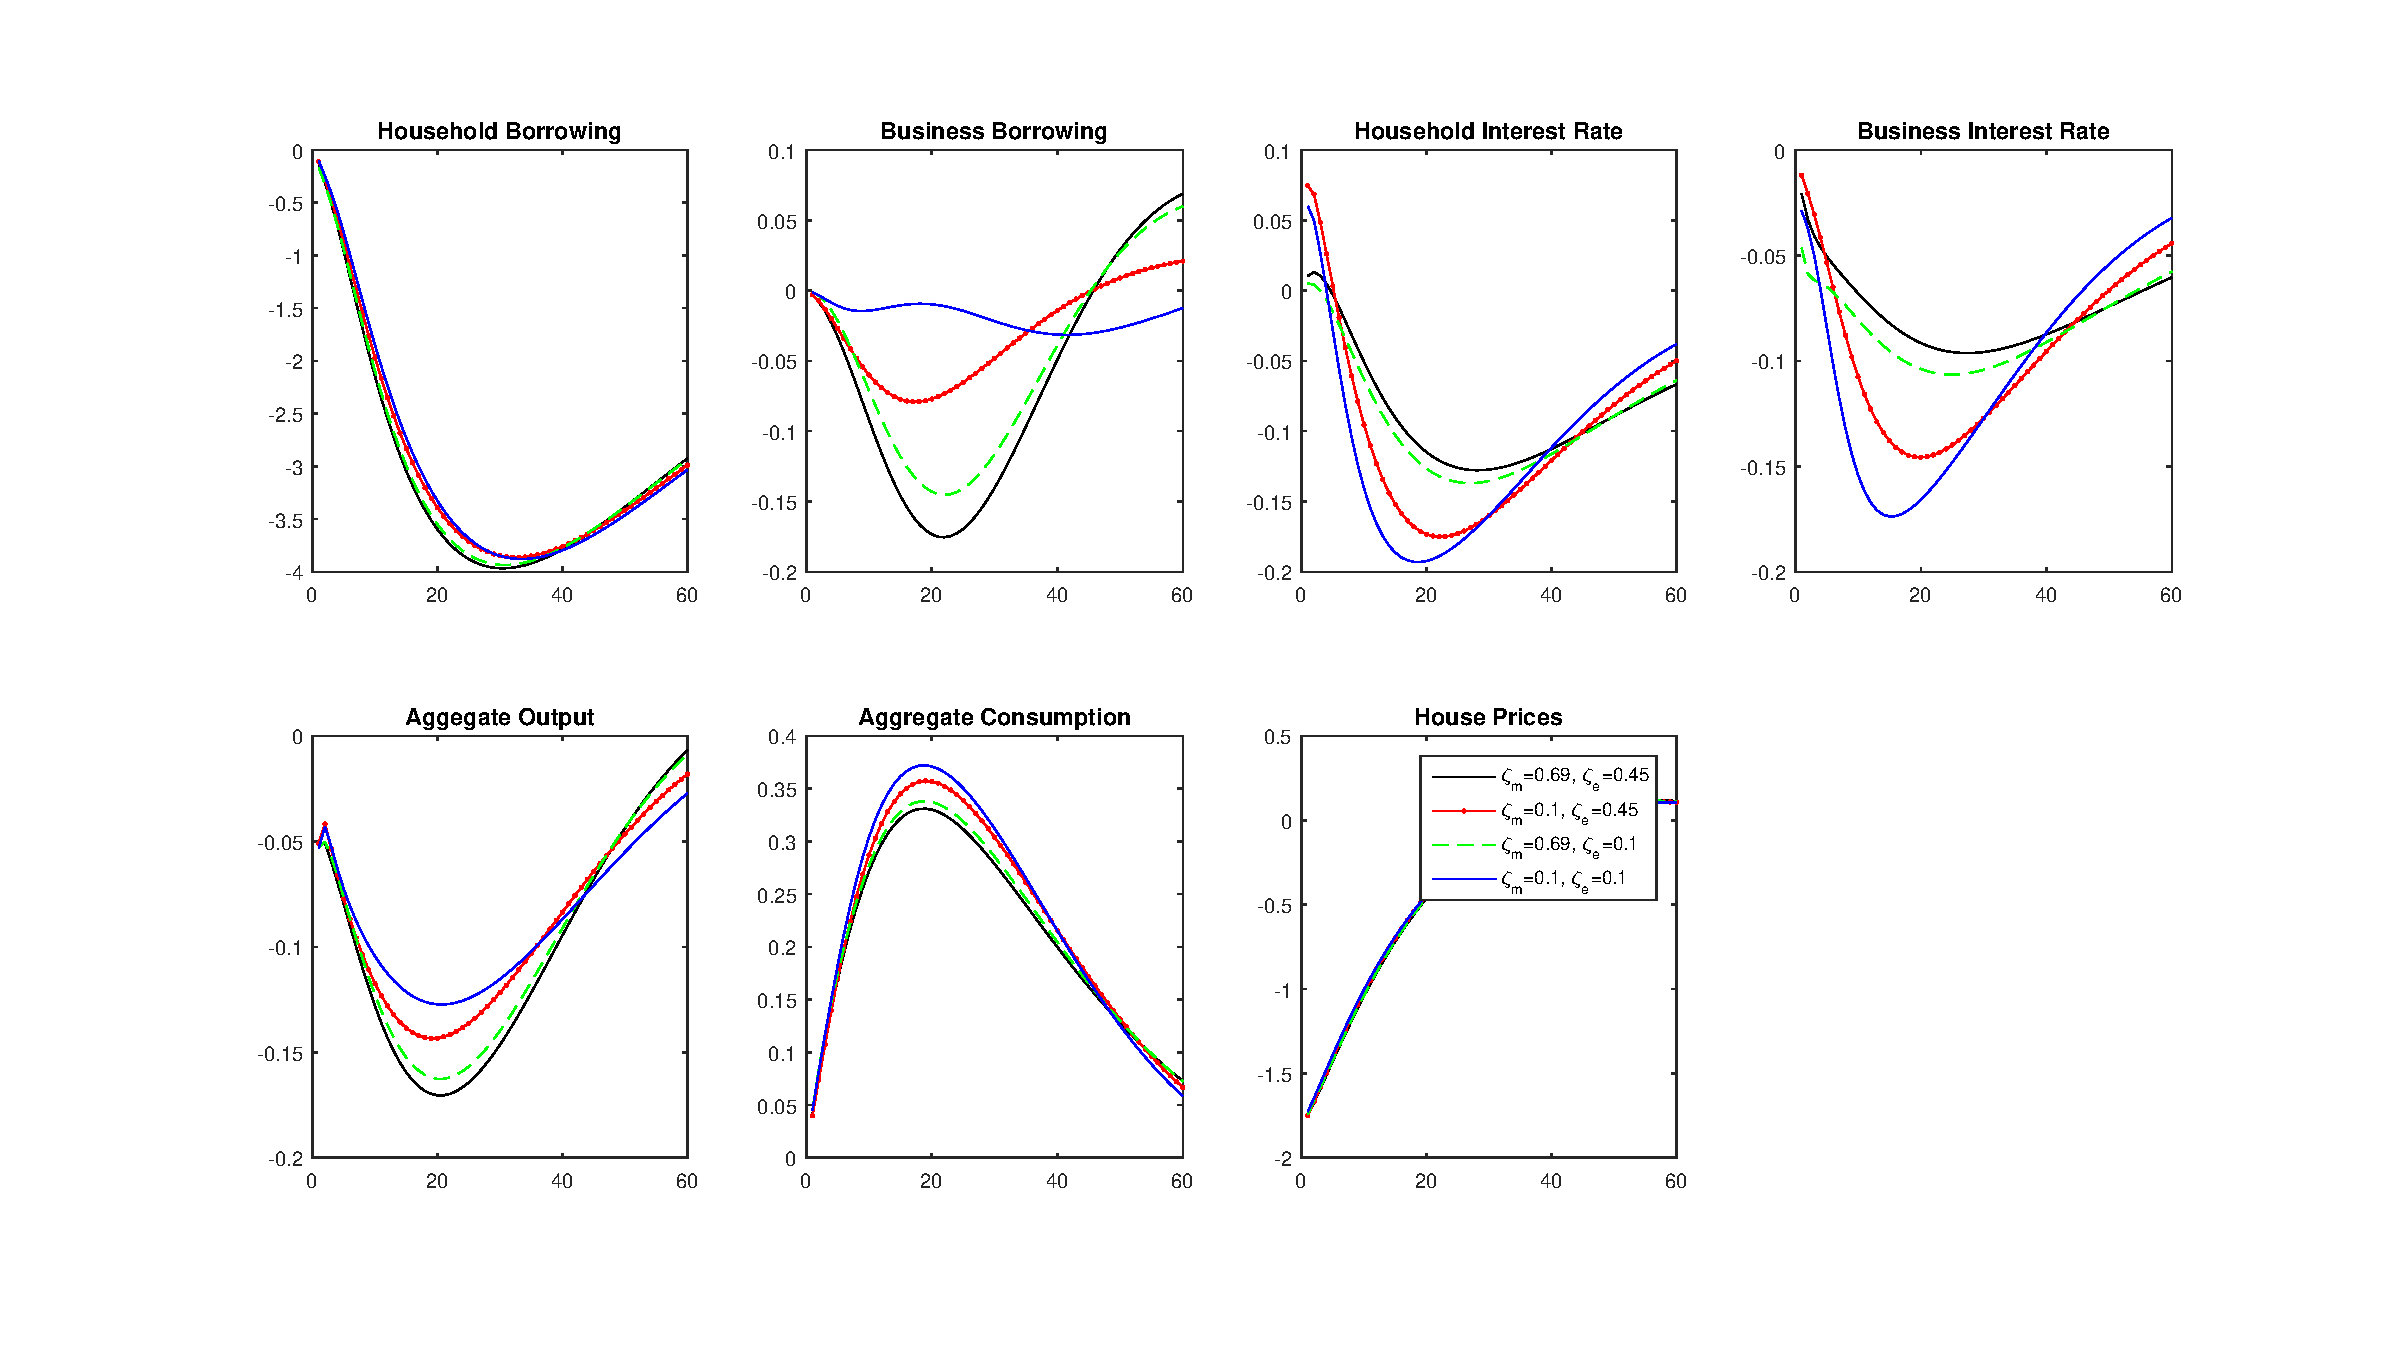
\includegraphics[scale=0.3]{stickinessJ.pdf}
\end{figure}



\end{frame}



\begin{frame}{Appendix-The effect of Interest rate Stickiness on Shock Transmission-II}

\begin{itemize}
\item A shock originating in the banking sector: \\transmission to both corporate and household sectors will depend on the degree of stickiness
\end{itemize}    

\begin{figure}[H]
\centering
\caption{Negative bank capital shock}
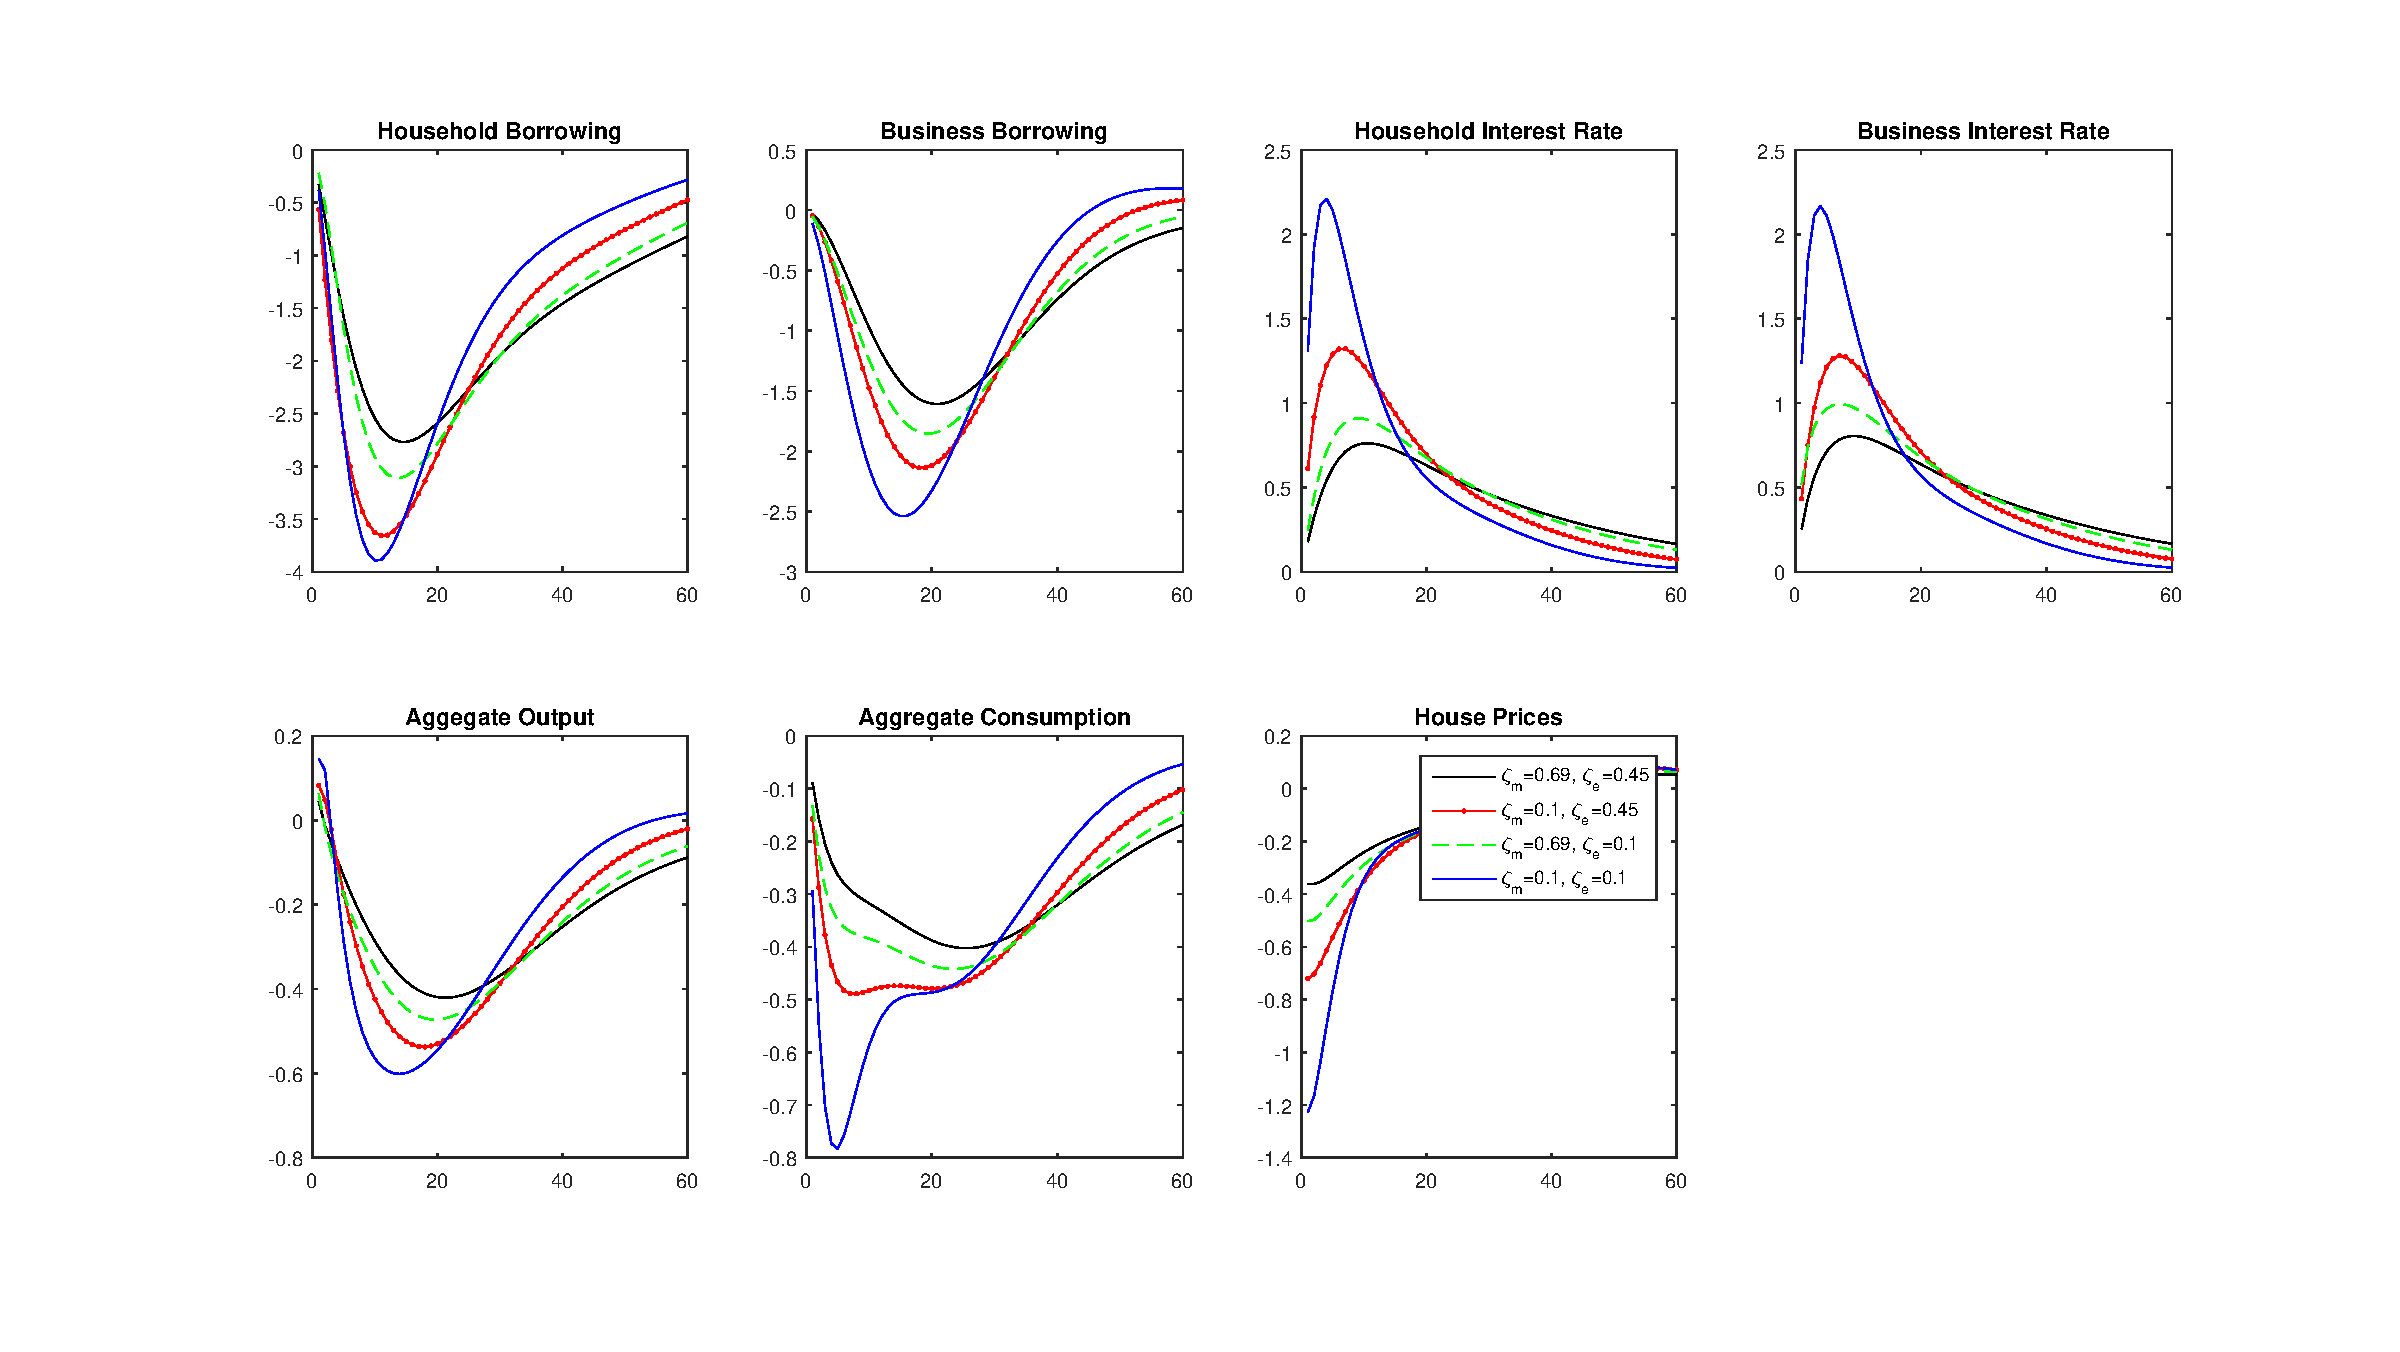
\includegraphics[scale=0.3]{stickinessCAB.pdf}
\end{figure}


\end{frame}

\

\end{comment}

\end{document}

